\documentclass[]{article}
\usepackage{lmodern}
\usepackage{amssymb,amsmath}
\usepackage{ifxetex,ifluatex}
\usepackage{fixltx2e} % provides \textsubscript
\ifnum 0\ifxetex 1\fi\ifluatex 1\fi=0 % if pdftex
  \usepackage[T1]{fontenc}
  \usepackage[utf8]{inputenc}
\else % if luatex or xelatex
  \ifxetex
    \usepackage{mathspec}
  \else
    \usepackage{fontspec}
  \fi
  \defaultfontfeatures{Ligatures=TeX,Scale=MatchLowercase}
\fi
% use upquote if available, for straight quotes in verbatim environments
\IfFileExists{upquote.sty}{\usepackage{upquote}}{}
% use microtype if available
\IfFileExists{microtype.sty}{%
\usepackage{microtype}
\UseMicrotypeSet[protrusion]{basicmath} % disable protrusion for tt fonts
}{}
\usepackage[margin=1in]{geometry}
\usepackage{hyperref}
\hypersetup{unicode=true,
            pdftitle={CUNY SPS DATA 621 - CTG5 - HW4},
            pdfauthor={Betsy Rosalen, Gabrielle Bartomeo, Jeremy O'Brien, Lidiia Tronina, Rose Koh},
            pdfborder={0 0 0},
            breaklinks=true}
\urlstyle{same}  % don't use monospace font for urls
\usepackage{longtable,booktabs}
\usepackage{graphicx,grffile}
\makeatletter
\def\maxwidth{\ifdim\Gin@nat@width>\linewidth\linewidth\else\Gin@nat@width\fi}
\def\maxheight{\ifdim\Gin@nat@height>\textheight\textheight\else\Gin@nat@height\fi}
\makeatother
% Scale images if necessary, so that they will not overflow the page
% margins by default, and it is still possible to overwrite the defaults
% using explicit options in \includegraphics[width, height, ...]{}
\setkeys{Gin}{width=\maxwidth,height=\maxheight,keepaspectratio}
\IfFileExists{parskip.sty}{%
\usepackage{parskip}
}{% else
\setlength{\parindent}{0pt}
\setlength{\parskip}{6pt plus 2pt minus 1pt}
}
\setlength{\emergencystretch}{3em}  % prevent overfull lines
\providecommand{\tightlist}{%
  \setlength{\itemsep}{0pt}\setlength{\parskip}{0pt}}
\setcounter{secnumdepth}{5}
% Redefines (sub)paragraphs to behave more like sections
\ifx\paragraph\undefined\else
\let\oldparagraph\paragraph
\renewcommand{\paragraph}[1]{\oldparagraph{#1}\mbox{}}
\fi
\ifx\subparagraph\undefined\else
\let\oldsubparagraph\subparagraph
\renewcommand{\subparagraph}[1]{\oldsubparagraph{#1}\mbox{}}
\fi

%%% Use protect on footnotes to avoid problems with footnotes in titles
\let\rmarkdownfootnote\footnote%
\def\footnote{\protect\rmarkdownfootnote}

%%% Change title format to be more compact
\usepackage{titling}

% Create subtitle command for use in maketitle
\newcommand{\subtitle}[1]{
  \posttitle{
    \begin{center}\large#1\end{center}
    }
}

\setlength{\droptitle}{-2em}

  \title{CUNY SPS DATA 621 - CTG5 - HW4}
    \pretitle{\vspace{\droptitle}\centering\huge}
  \posttitle{\par}
    \author{Betsy Rosalen, Gabrielle Bartomeo, Jeremy O'Brien, Lidiia Tronina, Rose
Koh}
    \preauthor{\centering\large\emph}
  \postauthor{\par}
      \predate{\centering\large\emph}
  \postdate{\par}
    \date{April 24th, 2019}

\usepackage{float}
\floatplacement{figure}{H}
\floatplacement{table}{H}
\usepackage{booktabs}
\usepackage{longtable}
\usepackage{array}
\usepackage{multirow}
\usepackage{wrapfig}
\usepackage{float}
\usepackage{colortbl}
\usepackage{pdflscape}
\usepackage{tabu}
\usepackage{threeparttable}
\usepackage{threeparttablex}
\usepackage[normalem]{ulem}
\usepackage{makecell}
\usepackage{xcolor}

\begin{document}
\maketitle

{
\setcounter{tocdepth}{2}
\tableofcontents
}
\newpage

\section{DATA EXPLORATION}\label{data-exploration}

In the pursuit of determining relationships between car crashes, their
costs, and factors that may play a role into each, a dataset containing
8,161 observations with 25 variables was explored, analyzed, and
modeled. This data came from an auto insurance company with each
observation representing one of their customers. Of the 25 variables,
two were target variables (car crashes and car costs), and the other 23
were predictors. \texttt{TARGET\_FLAG} is a binary variable where a
value of 1 indicates that the customer has made a claim related to a car
crash and a value of 0 indicates they have not. The other target
variable, \texttt{TARGET\_AMT}, is a continuous numerical variable whose
value is the payout amount of a claim, if any. The remaining variables
are split in their categorization; 13 are categorical and 10 are
numerical.

This data was utilized to compose and evaluate several types of models
with the following features:

\begin{itemize}
\tightlist
\item
  Logistic classification models that aim to predict the probability
  that a person crashes their car; and,
\item
  Multiple linear regression models that aim to predict the amount of
  money it will cost if the person does crash their car.
\end{itemize}

The intended use case for these models is actuarial in nature:
specifically, to calculate insurance rates commensurate with
policyholders' (or policy applicants') potential risk levels based on
attributes such as income, age, distance to work, tenure as customers,
so on and so forth.

\begin{table}

\caption{\label{tab:t1}Data Dictionary}
\centering
\begin{tabular}[t]{l|l|l}
\hline
VARIABLE & DEFINITION & TYPE\\
\hline
TARGET\_FLAG & car crash = 1, no car crash = 0 & binary categorical response\\
\hline
TARGET\_AMT & car crash cost = >0, no car crash = 0 & continuous numerical response\\
\hline
AGE & driver's age - very young/old tend to be risky & continuous numerical predictor\\
\hline
BLUEBOOK & \$ value of vehicle & continuous numerical predictor\\
\hline
CAR\_AGE & age of vehicle & continuous numerical predictor\\
\hline
CAR\_TYPE & type of car (6types) & categorical predictor\\
\hline
CAR\_USE & usage of car (commercial/private) & binary categorical predictor\\
\hline
CLM\_FREQ & number of claims past 5 years & discrete numerical predictor\\
\hline
EDUCATION & max education level (5types) & categorical predictor\\
\hline
HOMEKIDS & number of children at home & discrete numerical predictor\\
\hline
HOME\_VAL & \$ home value - home owners tend to drive more responsibly & continuous numerical predictor\\
\hline
INCOME & \$ income - rich people tend to get into fewer crashes & continuous numerical predictor\\
\hline
JOB & job category (8types, 1missing) - white collar tend to be safer & categorical predictor\\
\hline
KIDSDRIV & number of driving children - teenagers more likely to crash & discrete numerical predictor\\
\hline
MSTATUS & maritial status - married people drive more safely & catogerical predictor\\
\hline
MVR\_PTS & number of traffic tickets & continuous numerical predictor\\
\hline
OLDCLAIM & \$ total claims in the past 5 years & continuous numerical predictor\\
\hline
PARENT1 & single parent & binary categorical predictor\\
\hline
RED\_CAR & a red car & binary categorical predictor\\
\hline
REVOKED & license revoked (past 7 years) - more risky driver & binary categorical predictor\\
\hline
SEX & gender - woman may have less crashes than man & binary categorical predictor\\
\hline
TIF & time in force - number of years being customer & continuous numerical predictor\\
\hline
TRAVTIME & distance to work & continuous numerical predictor\\
\hline
URBANCITY & urban/rural & binary categorical predictor\\
\hline
YOJ & years on job - the longer they stay more safe & continuous numerical predictor\\
\hline
\end{tabular}
\end{table}

Inspection of the target variables reveals that where
\texttt{TARGET\_FLAG} has values of 0 (i.e., no claim),
\texttt{TARGET\_AMT} also has values of 0 (i.e., no payout) which is
logically consistent. Additionally even when the \texttt{TARGET\_FLAG}
is coded 1 indicating that a claim has been made, \texttt{TARGET\_AMT}
sometimes still has a value of zero indicating that not all claims
result in a payout.

\subsection{Summary Statistics}\label{summary-statistics}

Continuous and categorical variables were summarized separately for the
sake of clarity.

\begin{table}

\caption{\label{tab:t2}Summary statistics}
\centering
\begin{tabular}[t]{l|r|r|r|r|r|r}
\hline
  & n & min & mean & median & max & sd\\
\hline
TARGET\_AMT & 8161 & 0 & 1504.3 & 0 & 107586 & 4704.0\\
\hline
AGE & 8155 & 16 & 44.8 & 45 & 81 & 8.6\\
\hline
YOJ & 7707 & 0 & 10.5 & 11 & 23 & 4.1\\
\hline
INCOME & 7716 & 0 & 61898.1 & 54028 & 367030 & 47572.7\\
\hline
HOME\_VAL & 7697 & 0 & 154867.3 & 161160 & 885282 & 129123.8\\
\hline
TRAVTIME & 8161 & 5 & 33.5 & 33 & 142 & 15.9\\
\hline
BLUEBOOK & 8161 & 1500 & 15709.9 & 14440 & 69740 & 8419.7\\
\hline
TIF & 8161 & 1 & 5.3 & 4 & 25 & 4.2\\
\hline
OLDCLAIM & 8161 & 0 & 4037.1 & 0 & 57037 & 8777.1\\
\hline
MVR\_PTS & 8161 & 0 & 1.7 & 1 & 13 & 2.1\\
\hline
CAR\_AGE & 7651 & 0 & 8.3 & 8 & 28 & 5.7\\
\hline
\end{tabular}
\end{table}

\texttt{EDUCATION}, \texttt{JOB}, \texttt{CAR\_TYPE}, \texttt{KIDSDRIV},
\texttt{HOMEKIDS}, and \texttt{CLM\_FREQ} each comprise multiple
categories. On the other hand, \texttt{PARENT1}, \texttt{SEX},
\texttt{MSTATUS}, \texttt{CAR\_USE}, \texttt{RED\_CAR},
\texttt{REVOKED}, \texttt{URBANICITY} are all binaries.

\begin{table}

\caption{\label{tab:t3}Summary statistics for Categorical Variables}
\centering
\begin{tabular}[t]{l|l|l|l|l|l|l}
\hline
  &        EDUCATION &           JOB &        CAR\_TYPE & KIDSDRIV & HOMEKIDS & CLM\_FREQ\\
\hline
 & <High School:1203 & Blue Collar :1825 & Minivan    :2145 & 0:7180 & 0:5289 & 0:5009\\
\hline
 & Bachelors   :2242 & Clerical    :1271 & Panel Truck: 676 & 1: 636 & 1: 902 & 1: 997\\
\hline
 & Masters     :1658 & Professional:1117 & Pickup     :1389 & 2: 279 & 2:1118 & 2:1171\\
\hline
 & PhD         : 728 & Manager     : 988 & Sports Car : 907 & 3:  62 & 3: 674 & 3: 776\\
\hline
 & High School :2330 & Lawyer      : 835 & Van        : 750 & 4:   4 & 4: 164 & 4: 190\\
\hline
 & NA & Student     : 712 & SUV        :2294 & NA & 5:  14 & 5:  18\\
\hline
 & NA & (Other)     :1413 & NA & NA & NA & NA\\
\hline
\end{tabular}
\end{table}

\begin{table}

\caption{\label{tab:t4}Summary statistics for Binary Categorical Variables}
\centering
\begin{tabular}[t]{l|l|l|l|l|l|l|l}
\hline
  & PARENT1 & SEX & MSTATUS &       CAR\_USE & RED\_CAR & REVOKED & URBANICITY\\
\hline
 & No :7084 & M:3786 & Yes:4894 & Commercial:3029 & no :5783 & No :7161 & Urban:6492\\
\hline
 & Yes:1077 & F:4375 & No :3267 & Private   :5132 & yes:2378 & Yes:1000 & Rural:1669\\
\hline
\end{tabular}
\end{table}

\subsection{Variable Descriptions}\label{variable-descriptions}

\paragraph{KIDSDRIV}\label{kidsdriv}

\texttt{KIDSDRIV} is a categorical predictor with values ranging from 0
to 4. It shows heavy skew, with most cars having no kid drivers (value
of 0). Judging from the distribution, it appears that having a kid
driver results in higher probability of making a claim. Although it was
imported as a numeric variable, due to the small range of discrete
values it was transformed into a categorical variable with five ordered
levels.

\paragraph{AGE}\label{age}

\texttt{AGE} presents driver's age and shows a normal distribution
centered around 45 years. Looking at the boxplot of age below, there
does not appear to be a difference in the distribution between whether a
claim is made or not. Accordingly, \texttt{AGE} may not be helpful in
determining the probability of making a claim.

\paragraph{HOMEKIDS}\label{homekids}

\texttt{HOMEKIDS} is a predictor describing the number of children at
home ranging from 0 to 5. Although it was imported as a numeric
variable, due to the small range of discrete values it was transformed
into a categorical variable with six ordered levels.

\paragraph{YOJ}\label{yoj}

\texttt{YOJ} is a predictor describing the number of years on the job.
People who stay at a job for a longer time are believed to be safer
drivers. Apart from those who are unemployed (values of 0), \texttt{YOJ}
seems to show a normal distribution.

\paragraph{INCOME}\label{income}

\texttt{INCOME} is a heavily skewed predictor variable, suggesting that
outliers should be treated for modelling.

\paragraph{HOME\_VAL}\label{home_val}

\texttt{HOME\_VAL} is a home value predictor variable. In theory, home
owners tend to drive more responsibly. The difference between owners and
renters (values of 0) is visible in the summary statistics graph.

\paragraph{TRAVTIME}\label{travtime}

\texttt{TRAVTIME} is a predictor variable describing the distance to
work. Long drives to work would suggest greater risk of an accident and
claim. However, its graph shows a fairly normal distribution with a
slightly longer right tail and little difference between the two target
values, such that this variable may not be helpful in determining the
probability of making a claim.

\paragraph{BLUEBOOK}\label{bluebook}

\texttt{BLUEBOOK} is a predictor variable describing the value of the
car. The boxplot demonstrates that the lower the value of the car, the
higher the chance of making a claim. It is conceivable that
higher-priced cars are driven more carefully.

\paragraph{TIF}\label{tif}

\texttt{TIF} describes how long the customer has been with the insurance
company. Plots reveal that the longer the tenure of a policyholder, the
lower the likelihood of a claim - i.e.~safe drivers tend to remain so.

\paragraph{OLDCLAIM}\label{oldclaim}

\texttt{OLDCLAIM} is a predictor describing the value of claims made in
the past 5 years. It is very heavily skewed as most policyholders do not
make claims.

\paragraph{CLM\_FREQ}\label{clm_freq}

\texttt{CLM\_FREQ} is a predictor that describes the frequency of claims
in the past 5 years. It suggests that those who have made a claim in the
past 5 years are more likely to make another claim. Although it was
imported as a numeric variable, due to the small range of discrete
values it was transformed into a categorical variable with six ordered
levels.

\paragraph{MVR\_PTS}\label{mvr_pts}

\texttt{MVR\_PTS} is a predictor that describes motor vehicle record
points. The rationale is that more traffic tickets suggests less safe
driving and a higher likelihood of claims. It appears to be a highly
significant variable as seen in the boxplots below.

\paragraph{CAR\_AGE}\label{car_age}

\texttt{CAR\_AGE} describes the age of the policyholder's vehicle. One
value is -3, which must be an error - this is corrected to 0.

\paragraph{PARENT1}\label{parent1}

\texttt{PARENT1} indicates whether a policyholder is a single parent.
This variable has been factorized.

\paragraph{SEX}\label{sex}

\texttt{SEX} describes the gender of the driver. This variable has been
factorized. It does not appear to be significant variable in the
boxplots below.

\paragraph{MSTATUS}\label{mstatus}

\texttt{MSTATUS} describes the marital status of the policyholder. The
rationale is that married people drive more safely. This variable has
been factorized.

\paragraph{EDUCATION}\label{education}

\texttt{EDUCATION} describes the education level of the driver. This
variable is factorized. It may be correlated with \texttt{INCOME}.

\paragraph{JOB}\label{job}

\texttt{JOB} describes the type of job the driver has. This variable is
factorized. It may be correlated with INCOME. In theory policyholders
with white collar jobs tend to drive more safely.

\paragraph{CAR\_TYPE}\label{car_type}

\texttt{CAR\_TYPE} describes type of car. This variable is factorized.

\paragraph{CAR\_USE}\label{car_use}

\texttt{CAR\_USE} describes how the vehicle is used. Commercial vehicles
are driven more and may have an elevated probability of accidents and
claims. This variable is factorized.

\paragraph{RED\_CAR}\label{red_car}

\texttt{RED\_CAR} indicates whether the color of the vehicle is red. Red
vehicles, especially sports cars, are associated with riskier driving
and likelihood of claims. This variable is factorized.

\paragraph{REVOKED}\label{revoked}

\texttt{REVOKED} describes whether a policyholders license has been
revoked in the past 7 years. License revocation is associated with
riskier driving. This variable is factorized. The boxplot reveals that
policyholders who previously lost their license are more likely to file
claims.

\paragraph{URBANICITY}\label{urbanicity}

\texttt{URBANICITY} describes whether the driver lives in an urban area
or a rural area. This variable has been factorized.

\subsubsection{Summary Statistics
Graphs}\label{summary-statistics-graphs}

The shapes of the distributions of the continuous variables are very
similar for both target values for all predictors. There does not seem
to be a very large difference between those who file claims and those
who do not for any of the predictors.

\begin{figure}
\centering
\includegraphics{proj4_files/figure-latex/f1-1.pdf}
\caption{\label{fig:f1}Numeric Data Distributions as a Function of
TARGET\_FLAG}
\end{figure}

Examining the dispersion of claims between variables, it looks like
likelihoods are higher for drivers who are male, urban, blue collar,
unmarried, or parents; as well as for those with commercial vehicles or
a revoked license.

\begin{figure}
\centering
\includegraphics{proj4_files/figure-latex/f2-1.pdf}
\caption{\label{fig:f2}Categorical Data Distributions as a Function of
TARGET\_FLAG}
\end{figure}

The scale of the continuous variables' distributions are considerably
different and difficult to visualize together.

Scaling the distribution based on the standard deviation reveals that
outliers are very abundant for the continuous variables
\texttt{OLDCLAIM}, \texttt{INCOME}, \texttt{TRAV\_TIME},
\texttt{BLUEBOOK}, and to a lesser extent \texttt{HOME\_VAL} and
\texttt{TIF}. The variables that appear to have the most outliers are
\texttt{OLDCLAIM}, \texttt{BLUEBOOK}, \texttt{TRAVTIME}, and
\texttt{INCOME}.

\begin{figure}
\centering
\includegraphics{proj4_files/figure-latex/f3-1.pdf}
\caption{\label{fig:f3}Scaled Boxplots}
\end{figure}

All of the variables show varying levels of skew save \texttt{YOJ} and
\texttt{AGE} which appear the most normally distributed.

\begin{figure}
\centering
\includegraphics{proj4_files/figure-latex/f4-1.pdf}
\caption{\label{fig:f4}Linear relationship between each numeric predictor
and the target}
\end{figure}

\subsection{Linearity}\label{linearity}

\begin{figure}
\centering
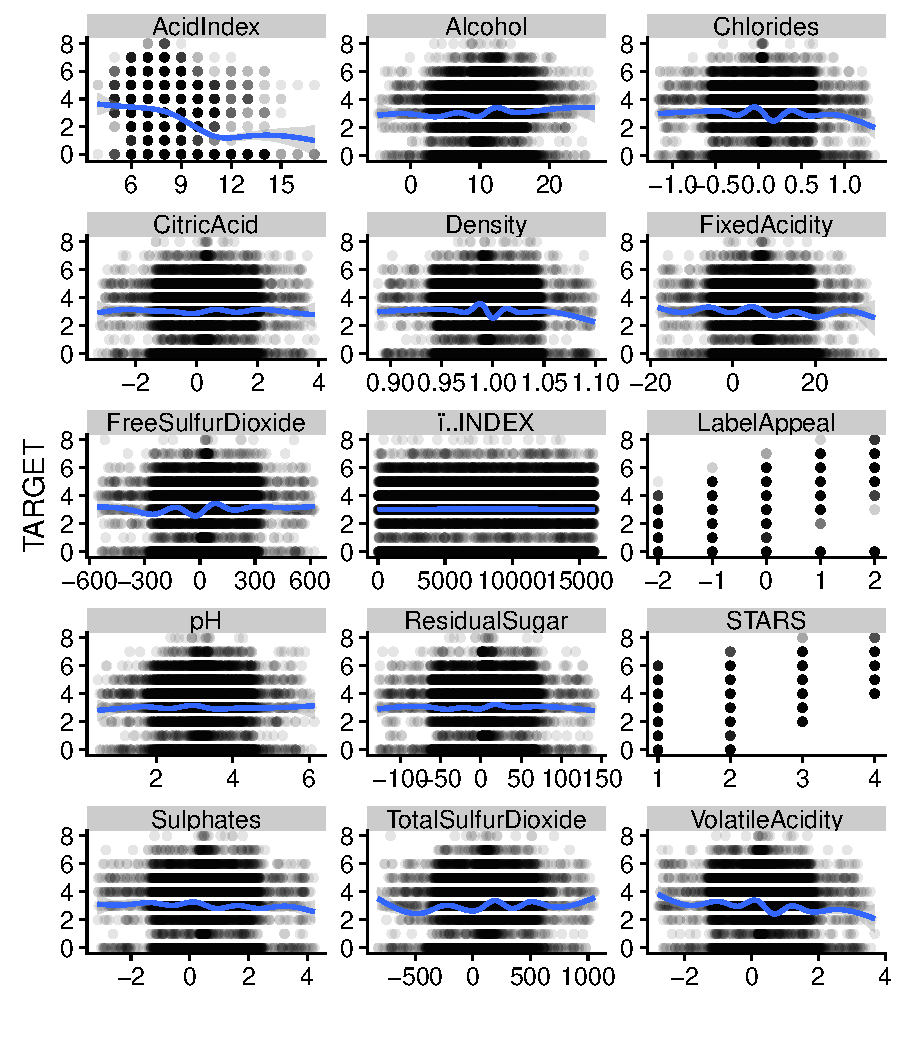
\includegraphics{proj4_files/figure-latex/f5-1.pdf}
\caption{\label{fig:f5}Scatter plot between numeric predictors and the
TARGET\_AMT, filtered for rows where TARGET\_AMT is greater than 0}
\end{figure}

The plotted numeric predictors with their raw values fail to show any
clear linear relationships with the \texttt{TARGET\_AMT} except for the
faintest of linearity in the \texttt{BLUEBOOK} variable.

{[}JO: DON'T THINK THE LOG TRANSFORM HAS HELPED - THINK WE SHOULD ADD{]}

{[}GAB: ADD WHAT? LOG DIDN'T HELP THOUGH YOU'RE RIGHT{]}

\subsubsection{Log Transformed Data}\label{log-transformed-data}

\begin{figure}
\centering
\includegraphics{proj4_files/figure-latex/f6.1-1.pdf}
\caption{(\#fig:f6.1)Scatter plot between log transformed numeric
predictors and the log transformed TARGET\_AMT filtered for rows where
TARGET\_AMT is greater than 0}
\end{figure}

In an attempt to distinguish the linearity of the variables alongside
the \texttt{TARGET\_AMT}, all numeric predictors and the
\texttt{TARGET\_AMT} underwent a log transformation. As a result, the
linearity of \texttt{BLUEBOOK} became more apparent, but there was no
obvious influence on the linearity of any of the other variables.

\subsubsection{Box-Cox}\label{box-cox}

Even though the linearity plots above don't show much improvement after
a log transformation, a Box-Cox plot shows that a log transformation is
recommended for the \texttt{TARGET\_AMT}.

\begin{figure}
\centering
\includegraphics{proj4_files/figure-latex/f6.2-1.pdf}
\caption{(\#fig:f6.2)Box-Cox Plot}
\end{figure}

\subsubsection{Square Root Transformed Predictors and Log Transformed
Target}\label{square-root-transformed-predictors-and-log-transformed-target}

A plot of each numerical predictor square root transformed plotted
against the log transformed \texttt{TARGET\_AMT} as recommended by the
Box-Cox plot still shows little improvement.

\begin{figure}
\centering
\includegraphics{proj4_files/figure-latex/f6.3-1.pdf}
\caption{(\#fig:f6.3)Scatter plot between square root transformed
numeric predictors and the square root transformed TARGET\_AMT filtered
for rows where TARGET\_AMT is greater than 0}
\end{figure}

\subsection{Missing Data}\label{missing-data}

\begin{figure}
\centering
\includegraphics{proj4_files/figure-latex/f7-1.pdf}
\caption{\label{fig:f7}Missing data}
\end{figure}

A number of variables are missing observations: \texttt{AGE},
\texttt{INCOME}, \texttt{YOJ}, \texttt{HOME\_VAL}, \texttt{CAR\_AGE}.
For \texttt{AGE}, the number is inconsequential, but the others range
between 5\% and 6\% of total. Approximately 21\% of the cases are
missing one of these variables, and an additional 2\% are missing more
than one. For this reason, we don't suspect latent factors can account
for the absences, and assume that these values are missing at random and
can be imputed when preparing the data for modeling.

\newpage

\section{DATA PREPARATION}\label{data-preparation}

\subsection{Missing Values}\label{missing-values}

{[}JO: WHAT'S THE DIFFERENCE BETWEEN THE M AND MAXIT VALUES (1 FOR AGE,
2 FOR OTHERS?){]}{[}GAB: CAN I KNOW THE ANSWER TO THIS TOO?{]}

To deal with missing data values for the variables \texttt{INCOME},
\texttt{YOJ}, \texttt{HOME\_VAL}, and \texttt{CAR\_AGE} - and to a
lesser extent \texttt{AGE} - the MICE (Multivariate Imputation By
Chained Equations) package was leveraged. The package assumes missing
values are missing at random and creates multiple imputations
(replacement values) for multivariate missing data using a a method
based on Fully Conditional Specification, where each incomplete variable
is imputed by a separate model. The method can impute mixes of
continuous, binary, unordered categorical and ordered categorical, and
continuous two-level data; and it can maintain consistency between
imputations by means of passive imputation. The quality of imputed
values was inspected using multiple diagnostic plots.

\begin{figure}
\centering
\includegraphics{proj4_files/figure-latex/f8-1.pdf}
\caption{\label{fig:f8}Difference between original and imputed data}
\end{figure}

The blue lines in the density plots above represent the original
distributions and the red lines include the imputed values. With the
exception of \texttt{AGE}, the distribution of the imputed values
accords with the distribution of pre-existing values. The imputed values
will be used for the four variables. Since \texttt{AGE} is missing only
0.07\% or 6 cases and displayed a strange change to the distrubution
using the mice package, it was imputed separately using median
imputation.

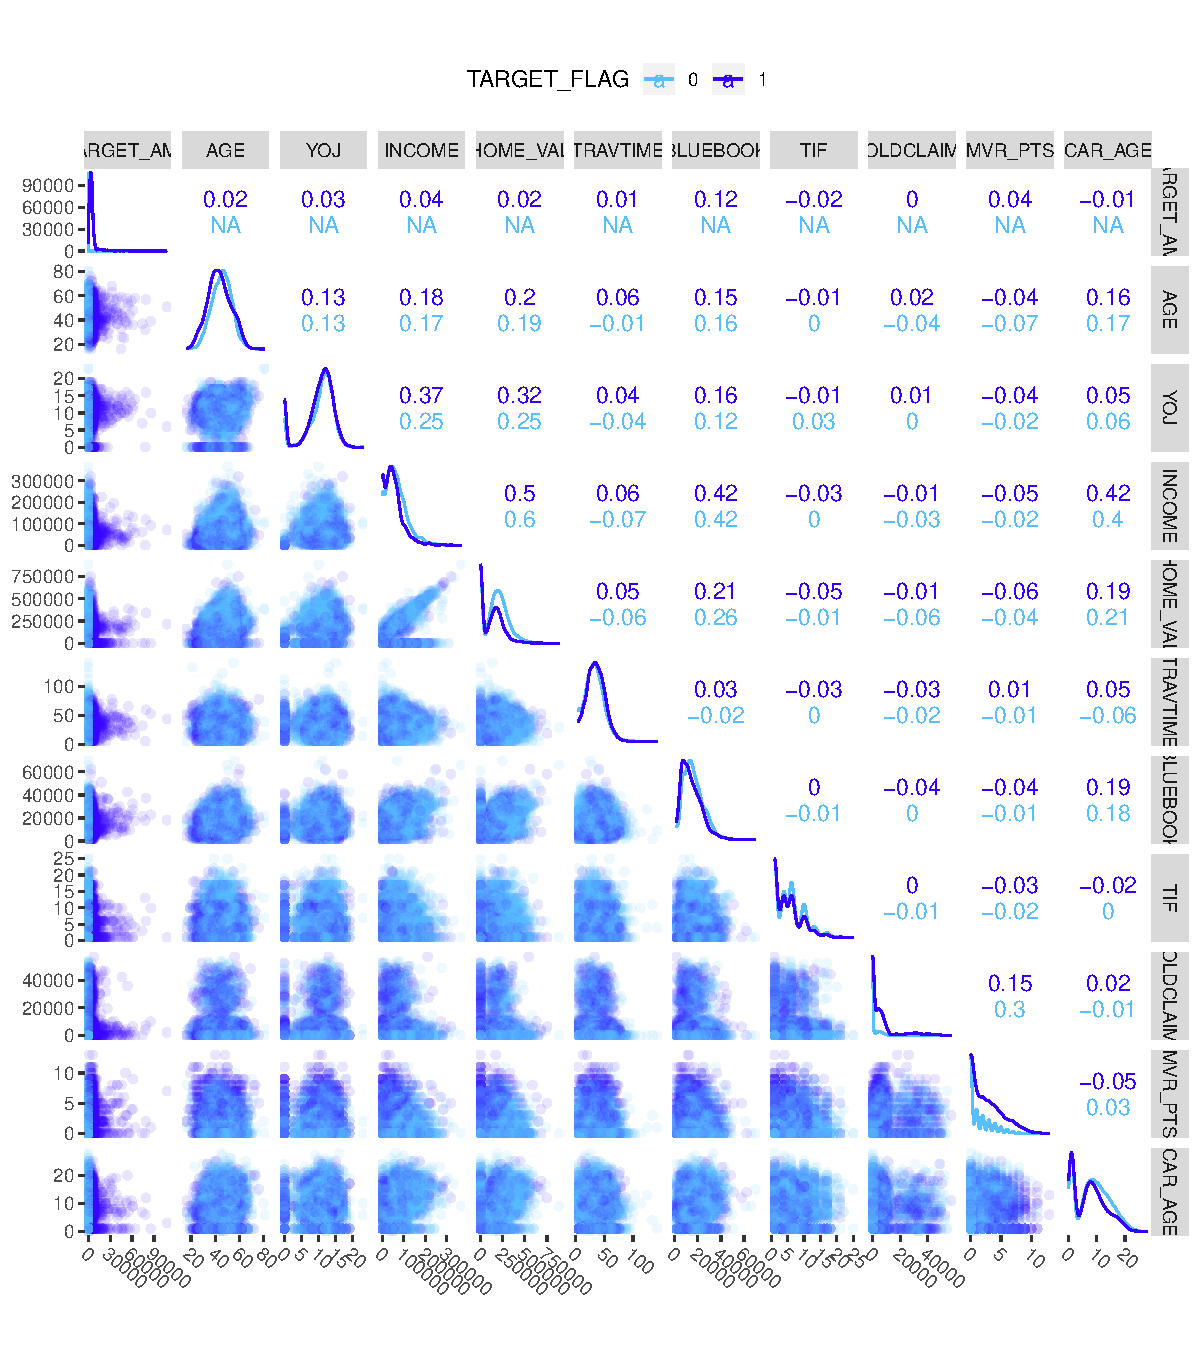
\includegraphics{proj4_files/figure-latex/f9-1.pdf}

Unsurprisingly, higher levels of \texttt{INCOME} are found with higher
values of \texttt{YOJ}; this also means more income is disposable, which
shows correlation with \texttt{HOME\_VAL} and \texttt{BLUEBOOK}.

Additionally, \texttt{MVR\_PTS} shows a positive correlation with
\texttt{OLDCLAIMS}.

\includegraphics{proj4_files/figure-latex/f10-1.pdf}

\newpage

\section{BUILD MODELS}\label{build-models}

\subsection{Classification Models: Models 1, 2 and
3}\label{classification-models-models-1-2-and-3}

The first three models use the predictor variables in binary logistic
models as inputs and interpret their contributions to predicting the
likelihood of a claim. We use \texttt{drop} and \texttt{MASS:stepAIC}
functions to judge which variables to remove, evaluating AIC statistics
as we go.

\subsubsection{Model 1 - Base model using categorical predictors
only}\label{model-1---base-model-using-categorical-predictors-only}

\begin{quote}
TARGET\_FLAG \textasciitilde{} PARENT1 + SEX + MSTATUS + EDUCATION + JOB
+ CAR\_TYPE + CAR\_USE + REVOKED + URBANICITY + KIDSDRIV + HOMEKIDS +
CLM\_FREQ
\end{quote}

For an easily interpretable model aimed at predicting TARGET\_FLAG,
inputs for Model 1 were restricted to categorical variables alone. The
AIC metric as well as the p-value and significance code suggests that
the \texttt{RED\_CAR} variable could be removed, so this predictor was
removed from model 1. Model 1 serves as a base model from which to
compare other models.

\begin{figure}
\centering
\includegraphics{proj4_files/figure-latex/f11-1.pdf}
\caption{\label{fig:f11}Model 1 ROC Curve}
\end{figure}

\begin{table}

\caption{\label{tab:t5}Area Under the Curve}
\centering
\begin{tabular}[t]{r}
\hline
x\\
\hline
0.8\\
\hline
\end{tabular}
\end{table}

\newpage

\subsubsection{Confusion Matrix}\label{confusion-matrix}

\begin{verbatim}
## Confusion Matrix and Statistics
## 
##           Reference
## Prediction    0    1
##          0 5471 1603
##          1  169  408
##                                               
##                Accuracy : 0.768               
##                  95% CI : (0.759, 0.778)      
##     No Information Rate : 0.737               
##     P-Value [Acc > NIR] : 0.000000000173      
##                                               
##                   Kappa : 0.224               
##  Mcnemar's Test P-Value : < 0.0000000000000002
##                                               
##             Sensitivity : 0.970               
##             Specificity : 0.203               
##          Pos Pred Value : 0.773               
##          Neg Pred Value : 0.707               
##               Precision : 0.773               
##                  Recall : 0.970               
##                      F1 : 0.861               
##              Prevalence : 0.737               
##          Detection Rate : 0.715               
##    Detection Prevalence : 0.925               
##       Balanced Accuracy : 0.586               
##                                               
##        'Positive' Class : 0                   
## 
\end{verbatim}

\begin{table}[!h]
\centering
\begin{tabular}{lr}
\toprule
\rowcolor{gray!6}  Observations & 7651\\
Dependent variable & TARGET\_FLAG\\
\rowcolor{gray!6}  Type & Generalized linear model\\
Family & binomial\\
\rowcolor{gray!6}  Link & logit\\
\bottomrule
\end{tabular}
\end{table}

\begin{table}[!h]
\centering
\begin{tabular}{lr}
\toprule
\rowcolor{gray!6}  $\chi^2$(37) & 1764.49\\
Pseudo-R² (Cragg-Uhler) & 0.30\\
\rowcolor{gray!6}  Pseudo-R² (McFadden) & 0.20\\
AIC & 7125.59\\
\rowcolor{gray!6}  BIC & 7389.41\\
\bottomrule
\end{tabular}
\end{table}

\begin{table}[!h]
\centering
\begin{threeparttable}
\begin{tabular}{lrrrrr}
\toprule
  & Est. & S.E. & z val. & p & VIF\\
\midrule
\rowcolor{gray!6}  (Intercept) & -1.68 & 0.23 & -7.27 & 0.00 & NA\\
PARENT1Yes & 0.22 & 0.12 & 1.78 & 0.07 & 2.34\\
\rowcolor{gray!6}  SEXF & -0.31 & 0.09 & -3.38 & 0.00 & 2.36\\
MSTATUSNo & 0.68 & 0.08 & 8.96 & 0.00 & 1.67\\
\rowcolor{gray!6}  EDUCATIONBachelors & -0.51 & 0.11 & -4.72 & 0.00 & 7.49\\
\addlinespace
EDUCATIONMasters & -0.41 & 0.16 & -2.51 & 0.01 & 7.49\\
\rowcolor{gray!6}  EDUCATIONPhD & -0.49 & 0.20 & -2.51 & 0.01 & 7.49\\
EDUCATIONHigh School & -0.03 & 0.10 & -0.35 & 0.73 & 7.49\\
\rowcolor{gray!6}  JOBClerical & 0.61 & 0.20 & 3.11 & 0.00 & 14.06\\
JOBDoctor & -0.27 & 0.26 & -1.03 & 0.30 & 14.06\\
\addlinespace
\rowcolor{gray!6}  JOBHome Maker & 0.72 & 0.20 & 3.63 & 0.00 & 14.06\\
JOBLawyer & 0.16 & 0.17 & 0.91 & 0.36 & 14.06\\
\rowcolor{gray!6}  JOBManager & -0.61 & 0.17 & -3.50 & 0.00 & 14.06\\
JOBProfessional & 0.24 & 0.18 & 1.35 & 0.18 & 14.06\\
\rowcolor{gray!6}  JOBStudent & 0.72 & 0.20 & 3.52 & 0.00 & 14.06\\
\addlinespace
JOBBlue Collar & 0.43 & 0.19 & 2.28 & 0.02 & 14.06\\
\rowcolor{gray!6}  CAR\_TYPEPanel Truck & 0.21 & 0.14 & 1.49 & 0.14 & 3.71\\
CAR\_TYPEPickup & 0.59 & 0.10 & 5.79 & 0.00 & 3.71\\
\rowcolor{gray!6}  CAR\_TYPESports Car & 1.22 & 0.12 & 9.84 & 0.00 & 3.71\\
CAR\_TYPEVan & 0.40 & 0.12 & 3.22 & 0.00 & 3.71\\
\addlinespace
\rowcolor{gray!6}  CAR\_TYPESUV & 0.95 & 0.10 & 9.06 & 0.00 & 3.71\\
CAR\_USEPrivate & -0.74 & 0.09 & -7.96 & 0.00 & 2.47\\
\rowcolor{gray!6}  REVOKEDYes & 0.74 & 0.08 & 9.10 & 0.00 & 1.01\\
URBANICITYRural & -2.20 & 0.11 & -19.34 & 0.00 & 1.11\\
\rowcolor{gray!6}  KIDSDRIV1 & 0.40 & 0.11 & 3.51 & 0.00 & 1.54\\
\addlinespace
KIDSDRIV2 & 0.69 & 0.16 & 4.20 & 0.00 & 1.54\\
\rowcolor{gray!6}  KIDSDRIV3 & 0.86 & 0.32 & 2.72 & 0.01 & 1.54\\
KIDSDRIV4 & -11.10 & 204.58 & -0.05 & 0.96 & 1.54\\
\rowcolor{gray!6}  HOMEKIDS1 & 0.34 & 0.11 & 3.01 & 0.00 & 2.65\\
HOMEKIDS2 & 0.28 & 0.11 & 2.51 & 0.01 & 2.65\\
\addlinespace
\rowcolor{gray!6}  HOMEKIDS3 & 0.27 & 0.13 & 2.09 & 0.04 & 2.65\\
HOMEKIDS4 & 0.05 & 0.21 & 0.26 & 0.80 & 2.65\\
\rowcolor{gray!6}  HOMEKIDS5 & 0.03 & 0.69 & 0.05 & 0.96 & 2.65\\
CLM\_FREQ1 & 0.64 & 0.09 & 7.41 & 0.00 & 1.06\\
\rowcolor{gray!6}  CLM\_FREQ2 & 0.68 & 0.08 & 8.51 & 0.00 & 1.06\\
\addlinespace
CLM\_FREQ3 & 0.67 & 0.09 & 7.08 & 0.00 & 1.06\\
\rowcolor{gray!6}  CLM\_FREQ4 & 0.97 & 0.17 & 5.61 & 0.00 & 1.06\\
CLM\_FREQ5 & 1.00 & 0.55 & 1.84 & 0.07 & 1.06\\
\bottomrule
\end{tabular}
\begin{tablenotes}
\item Standard errors: MLE
\end{tablenotes}
\end{threeparttable}
\end{table}

\newpage

\subsubsection{Model 2 - Refined base model plus numerical
predictors}\label{model-2---refined-base-model-plus-numerical-predictors}

\begin{quote}
TARGET\_FLAG \textasciitilde{} MSTATUS + EDUCATION\_Bachelors +
JOB\_Clerical + JOB\_Manager + CAR\_TYPE + CAR\_USE + REVOKED +
URBANICITY + KIDSDRIV + HOMEKIDS + CLM\_FREQ + INCOME + HOME\_VAL +
TRAVTIME + BLUEBOOK + TIF + OLDCLAIM + MVR\_PTS,
\end{quote}

Building on model 1, model 2 excludes the \texttt{RED\_CAR} variable and
adds in all of the numerical variables to see if they add value to our
model. After the initial model statistics were examined we then further
refined the model by removing \texttt{AGE}, \texttt{CAR\_AGE},
\texttt{SEX}, \texttt{YOJ}, and \texttt{PARENT1} due to low p-value
significance. \texttt{EDUCATION}, and \texttt{JOB} were only significant
if the education was `Bachelors' or if the job was `Manager', so two new
binary variables, \texttt{EDUCATION\_Bachelors} and
\texttt{JOB\_Manager} were added to the dataset indicating yes or no for
these specific education and job values.

\begin{figure}
\centering
\includegraphics{proj4_files/figure-latex/f12-1.pdf}
\caption{\label{fig:f12}Model 3 ROC Curve}
\end{figure}

\begin{table}

\caption{\label{tab:t7}Area Under the Curve}
\centering
\begin{tabular}[t]{r}
\hline
x\\
\hline
0.81\\
\hline
\end{tabular}
\end{table}

\subsubsection{Confusion Matrix}\label{confusion-matrix-1}

\begin{verbatim}
## Confusion Matrix and Statistics
## 
##           Reference
## Prediction    0    1
##          0 5455 1505
##          1  185  506
##                                              
##                Accuracy : 0.779              
##                  95% CI : (0.77, 0.788)      
##     No Information Rate : 0.737              
##     P-Value [Acc > NIR] : <0.0000000000000002
##                                              
##                   Kappa : 0.277              
##  Mcnemar's Test P-Value : <0.0000000000000002
##                                              
##             Sensitivity : 0.967              
##             Specificity : 0.252              
##          Pos Pred Value : 0.784              
##          Neg Pred Value : 0.732              
##               Precision : 0.784              
##                  Recall : 0.967              
##                      F1 : 0.866              
##              Prevalence : 0.737              
##          Detection Rate : 0.713              
##    Detection Prevalence : 0.910              
##       Balanced Accuracy : 0.609              
##                                              
##        'Positive' Class : 0                  
## 
\end{verbatim}

\begin{table}[!h]
\centering
\begin{tabular}{lr}
\toprule
\rowcolor{gray!6}  Observations & 7651\\
Dependent variable & TARGET\_FLAG\\
\rowcolor{gray!6}  Type & Generalized linear model\\
Family & binomial\\
\rowcolor{gray!6}  Link & logit\\
\bottomrule
\end{tabular}
\end{table}

\begin{table}[!h]
\centering
\begin{tabular}{lr}
\toprule
\rowcolor{gray!6}  $\chi^2$(33) & 1986.84\\
Pseudo-R² (Cragg-Uhler) & 0.33\\
\rowcolor{gray!6}  Pseudo-R² (McFadden) & 0.23\\
AIC & 6895.24\\
\rowcolor{gray!6}  BIC & 7131.28\\
\bottomrule
\end{tabular}
\end{table}

\begin{table}[!h]
\centering
\begin{threeparttable}
\begin{tabular}{lrrrrr}
\toprule
  & Est. & S.E. & z val. & p & VIF\\
\midrule
\rowcolor{gray!6}  (Intercept) & -0.96 & 0.16 & -6.18 & 0.00 & NA\\
MSTATUSNo & 0.64 & 0.08 & 8.55 & 0.00 & 1.55\\
\rowcolor{gray!6}  EDUCATION\_BachelorsTRUE & -0.27 & 0.07 & -3.89 & 0.00 & 1.05\\
JOB\_ClericalTRUE & 0.26 & 0.09 & 3.05 & 0.00 & 1.16\\
\rowcolor{gray!6}  JOB\_ManagerTRUE & -0.77 & 0.11 & -6.79 & 0.00 & 1.08\\
\addlinespace
CAR\_TYPEPanel Truck & 0.52 & 0.15 & 3.51 & 0.00 & 2.23\\
\rowcolor{gray!6}  CAR\_TYPEPickup & 0.46 & 0.10 & 4.50 & 0.00 & 2.23\\
CAR\_TYPESports Car & 0.93 & 0.11 & 8.47 & 0.00 & 2.23\\
\rowcolor{gray!6}  CAR\_TYPEVan & 0.54 & 0.12 & 4.37 & 0.00 & 2.23\\
CAR\_TYPESUV & 0.67 & 0.09 & 7.61 & 0.00 & 2.23\\
\addlinespace
\rowcolor{gray!6}  CAR\_USEPrivate & -0.90 & 0.07 & -12.10 & 0.00 & 1.52\\
REVOKEDYes & 0.95 & 0.10 & 9.96 & 0.00 & 1.36\\
\rowcolor{gray!6}  URBANICITYRural & -2.29 & 0.12 & -19.72 & 0.00 & 1.13\\
KIDSDRIV1 & 0.42 & 0.12 & 3.64 & 0.00 & 1.53\\
\rowcolor{gray!6}  KIDSDRIV2 & 0.71 & 0.17 & 4.25 & 0.00 & 1.53\\
\addlinespace
KIDSDRIV3 & 0.74 & 0.32 & 2.29 & 0.02 & 1.53\\
\rowcolor{gray!6}  KIDSDRIV4 & -11.57 & 199.91 & -0.06 & 0.95 & 1.53\\
HOMEKIDS1 & 0.42 & 0.10 & 4.36 & 0.00 & 1.60\\
\rowcolor{gray!6}  HOMEKIDS2 & 0.36 & 0.10 & 3.77 & 0.00 & 1.60\\
HOMEKIDS3 & 0.36 & 0.12 & 3.08 & 0.00 & 1.60\\
\addlinespace
\rowcolor{gray!6}  HOMEKIDS4 & 0.21 & 0.21 & 1.03 & 0.30 & 1.60\\
HOMEKIDS5 & 0.25 & 0.70 & 0.36 & 0.72 & 1.60\\
\rowcolor{gray!6}  CLM\_FREQ1 & 0.58 & 0.10 & 5.68 & 0.00 & 1.87\\
CLM\_FREQ2 & 0.67 & 0.10 & 6.85 & 0.00 & 1.87\\
\rowcolor{gray!6}  CLM\_FREQ3 & 0.62 & 0.11 & 5.67 & 0.00 & 1.87\\
\addlinespace
CLM\_FREQ4 & 0.81 & 0.18 & 4.50 & 0.00 & 1.87\\
\rowcolor{gray!6}  CLM\_FREQ5 & 1.14 & 0.56 & 2.04 & 0.04 & 1.87\\
INCOME & -0.00 & 0.00 & -5.97 & 0.00 & 1.84\\
\rowcolor{gray!6}  HOME\_VAL & -0.00 & 0.00 & -3.34 & 0.00 & 1.94\\
TRAVTIME & 0.01 & 0.00 & 7.67 & 0.00 & 1.04\\
\addlinespace
\rowcolor{gray!6}  BLUEBOOK & -0.00 & 0.00 & -4.73 & 0.00 & 1.76\\
TIF & -0.06 & 0.01 & -7.39 & 0.00 & 1.01\\
\rowcolor{gray!6}  OLDCLAIM & -0.00 & 0.00 & -4.62 & 0.00 & 1.89\\
MVR\_PTS & 0.10 & 0.01 & 6.83 & 0.00 & 1.24\\
\bottomrule
\end{tabular}
\begin{tablenotes}
\item Standard errors: MLE
\end{tablenotes}
\end{threeparttable}
\end{table}

\newpage

\subsubsection{Model 3 - Binary logistic
model}\label{model-3---binary-logistic-model}

Model 3 takes a similar approach to model 2 by incorporating all numeric
predictor variables plus the categorical predictors that were found to
be significant in the previous model. Skewed numeric predictors
(\texttt{BLUEBOOK}, \texttt{CAR\_AGE}, \texttt{HOME\_VAL},
\texttt{INCOME}, \texttt{MVR\_PTS}, \texttt{OLDCLAIM}, \texttt{TIF}, and
\texttt{TRAVTIME}, ) were log transformed and added to the model as
additional predictors. \texttt{AGE} and \texttt{YOJ} were not included
since they were already normally distributed and determined not to be
significant in the previous models. The model was then refined through
backward elimination.

\paragraph{Original Model}\label{original-model}

\begin{quote}
TARGET\_FLAG \textasciitilde{} MSTATUS + EDUCATION\_Bachelors +
JOB\_Clerical + JOB\_Manager + CAR\_TYPE + CAR\_USE + REVOKED +
URBANICITY + KIDSDRIV + HOMEKIDS + CLM\_FREQ + BLUEBOOK + CAR\_AGE +
HOME\_VAL + INCOME + MVR\_PTS + OLDCLAIM + TIF + TRAVTIME +
log(BLUEBOOK) + log(CAR\_AGE+1) + log(HOME\_VAL+1) + log(INCOME+1) +
log(MVR\_PTS+1) + log(OLDCLAIM+1) + log(TIF) + log(TRAVTIME),
\end{quote}

\paragraph{Model after backward elimination
process}\label{model-after-backward-elimination-process}

\begin{quote}
TARGET\_FLAG \textasciitilde{} MSTATUS + EDUCATION\_Bachelors +
JOB\_Clerical + JOB\_Manager + CAR\_TYPE + CAR\_USE + REVOKED +
URBANICITY + KIDSDRIV + HOMEKIDS + CAR\_AGE + HOME\_VAL + INCOME +
MVR\_PTS + OLDCLAIM + log(BLUEBOOK) + log(INCOME+1) + log(OLDCLAIM+1) +
log(TIF) + log(TRAVTIME),
\end{quote}

\begin{figure}
\centering
\includegraphics{proj4_files/figure-latex/f13-1.pdf}
\caption{\label{fig:f13}Model 4 ROC Curve}
\end{figure}

\begin{table}

\caption{\label{tab:t9}Area Under the Curve}
\centering
\begin{tabular}[t]{r}
\hline
x\\
\hline
0.82\\
\hline
\end{tabular}
\end{table}

\subsubsection{Confusion Matrix}\label{confusion-matrix-2}

\begin{verbatim}
## Confusion Matrix and Statistics
## 
##           Reference
## Prediction    0    1
##          0 5449 1491
##          1  191  520
##                                              
##                Accuracy : 0.78               
##                  95% CI : (0.771, 0.789)     
##     No Information Rate : 0.737              
##     P-Value [Acc > NIR] : <0.0000000000000002
##                                              
##                   Kappa : 0.284              
##  Mcnemar's Test P-Value : <0.0000000000000002
##                                              
##             Sensitivity : 0.966              
##             Specificity : 0.259              
##          Pos Pred Value : 0.785              
##          Neg Pred Value : 0.731              
##               Precision : 0.785              
##                  Recall : 0.966              
##                      F1 : 0.866              
##              Prevalence : 0.737              
##          Detection Rate : 0.712              
##    Detection Prevalence : 0.907              
##       Balanced Accuracy : 0.612              
##                                              
##        'Positive' Class : 0                  
## 
\end{verbatim}

\newpage

\begin{table}[!h]
\centering
\begin{tabular}{lr}
\toprule
\rowcolor{gray!6}  Observations & 7651\\
Dependent variable & TARGET\_FLAG\\
\rowcolor{gray!6}  Type & Generalized linear model\\
Family & binomial\\
\rowcolor{gray!6}  Link & logit\\
\bottomrule
\end{tabular}
\end{table}

\begin{table}[!h]
\centering
\begin{tabular}{lr}
\toprule
\rowcolor{gray!6}  $\chi^2$(31) & 2017.05\\
Pseudo-R² (Cragg-Uhler) & 0.34\\
\rowcolor{gray!6}  Pseudo-R² (McFadden) & 0.23\\
AIC & 6861.02\\
\rowcolor{gray!6}  BIC & 7083.19\\
\bottomrule
\end{tabular}
\end{table}

\begin{table}[!h]
\centering
\begin{threeparttable}
\begin{tabular}{lrrrrr}
\toprule
  & Est. & S.E. & z val. & p & VIF\\
\midrule
\rowcolor{gray!6}  (Intercept) & 1.13 & 0.57 & 1.96 & 0.05 & NA\\
MSTATUSNo & 0.66 & 0.08 & 8.79 & 0.00 & 1.55\\
\rowcolor{gray!6}  EDUCATION\_BachelorsTRUE & -0.26 & 0.07 & -3.61 & 0.00 & 1.05\\
JOB\_ClericalTRUE & 0.28 & 0.09 & 3.01 & 0.00 & 1.30\\
\rowcolor{gray!6}  JOB\_ManagerTRUE & -0.73 & 0.11 & -6.49 & 0.00 & 1.08\\
\addlinespace
CAR\_TYPEPanel Truck & 0.45 & 0.14 & 3.17 & 0.00 & 1.96\\
\rowcolor{gray!6}  CAR\_TYPEPickup & 0.46 & 0.10 & 4.56 & 0.00 & 1.96\\
CAR\_TYPESports Car & 0.90 & 0.11 & 8.12 & 0.00 & 1.96\\
\rowcolor{gray!6}  CAR\_TYPEVan & 0.55 & 0.12 & 4.46 & 0.00 & 1.96\\
CAR\_TYPESUV & 0.67 & 0.09 & 7.64 & 0.00 & 1.96\\
\addlinespace
\rowcolor{gray!6}  CAR\_USEPrivate & -0.89 & 0.08 & -11.69 & 0.00 & 1.57\\
REVOKEDYes & 0.97 & 0.10 & 10.10 & 0.00 & 1.37\\
\rowcolor{gray!6}  URBANICITYRural & -2.31 & 0.12 & -19.87 & 0.00 & 1.13\\
KIDSDRIV1 & 0.44 & 0.12 & 3.73 & 0.00 & 1.53\\
\rowcolor{gray!6}  KIDSDRIV2 & 0.72 & 0.17 & 4.30 & 0.00 & 1.53\\
\addlinespace
KIDSDRIV3 & 0.76 & 0.33 & 2.32 & 0.02 & 1.53\\
\rowcolor{gray!6}  KIDSDRIV4 & -11.62 & 190.55 & -0.06 & 0.95 & 1.53\\
HOMEKIDS1 & 0.41 & 0.10 & 4.17 & 0.00 & 1.61\\
\rowcolor{gray!6}  HOMEKIDS2 & 0.33 & 0.10 & 3.44 & 0.00 & 1.61\\
HOMEKIDS3 & 0.34 & 0.12 & 2.84 & 0.00 & 1.61\\
\addlinespace
\rowcolor{gray!6}  HOMEKIDS4 & 0.15 & 0.21 & 0.72 & 0.47 & 1.61\\
HOMEKIDS5 & 0.21 & 0.70 & 0.30 & 0.76 & 1.61\\
\rowcolor{gray!6}  CAR\_AGE & -0.02 & 0.01 & -3.15 & 0.00 & 1.30\\
HOME\_VAL & -0.00 & 0.00 & -3.05 & 0.00 & 1.97\\
\rowcolor{gray!6}  INCOME & -0.00 & 0.00 & -3.08 & 0.00 & 2.57\\
\addlinespace
MVR\_PTS & 0.10 & 0.01 & 6.74 & 0.00 & 1.24\\
\rowcolor{gray!6}  OLDCLAIM & -0.00 & 0.00 & -5.59 & 0.00 & 2.33\\
log(BLUEBOOK) & -0.32 & 0.06 & -5.51 & 0.00 & 1.48\\
\rowcolor{gray!6}  log(INCOME + 1) & -0.03 & 0.01 & -2.82 & 0.00 & 1.75\\
log(OLDCLAIM + 1) & 0.08 & 0.01 & 8.20 & 0.00 & 2.22\\
\addlinespace
\rowcolor{gray!6}  log(TIF) & -0.23 & 0.03 & -7.26 & 0.00 & 1.01\\
log(TRAVTIME) & 0.41 & 0.05 & 7.60 & 0.00 & 1.03\\
\bottomrule
\end{tabular}
\begin{tablenotes}
\item Standard errors: MLE
\end{tablenotes}
\end{threeparttable}
\end{table}

\newpage

\subsection{Regression Models: Models 4, 5, and
6}\label{regression-models-models-4-5-and-6}

The next two models are multiple linear regression models aimed at
predicting the value of claims based on different approaches, including
constraining the cases based on \texttt{TARGET\_FLAG} (i.e.~based on
whether or not a claim was filed) and different approaches to selecting
explanatory variables.

23 lines were removed where \texttt{TARGET\_AMT} greater than \$45,000;
these lines had a \texttt{BLUEBOOK} value far less than the car crash
cost. A new variable \texttt{mileage} was created based on
\texttt{TRAVTIME} and \texttt{CAR\_AGE}.

\subsubsection{Model 4 - Multiple linear regression
model}\label{model-4---multiple-linear-regression-model}

Model 4 is a multiple linear regression model built only on cases with
claims where \texttt{TARGET\_FLAG} equals 1. The model is refined using
stepwise elimination. From the model summary it can be observed that the
Adjusted R-squared value is very low at 0.04.

\begin{quote}
TARGET\_AMT \textasciitilde{} KIDSDRIV + log(AGE) + AGE + HOMEKIDS + YOJ
+ log(INCOME + 0.00000000000001) + INCOME + CAR\_AGE + log(mileage) +
log(BLUEBOOK) + BLUEBOOK + TIF + log(OLDCLAIM + 0.00000000000001) +
OLDCLAIM + CLM\_FREQ + MVR\_PTS + CAR\_AGE + PARENT1 + SEX +
EDUCATION\_Bachelors + JOB\_Clerical + JOB\_Manager + CAR\_TYPE +
REVOKED + URBANICITY + MSTATUS + CAR\_USE
\end{quote}

\begin{figure}
\centering
\includegraphics{proj4_files/figure-latex/f14-1.pdf}
\caption{\label{fig:f14}Model 4 Diagnostic Plots}
\end{figure}

\begin{table}[!h]
\centering
\begin{tabular}{lr}
\toprule
\rowcolor{gray!6}  Observations & 1988\\
Dependent variable & TARGET\_AMT\\
\rowcolor{gray!6}  Type & OLS linear regression\\
\bottomrule
\end{tabular}
\end{table}

\begin{table}[!h]
\centering
\begin{tabular}{lr}
\toprule
\rowcolor{gray!6}  F(40,1947) & 1.44\\
R² & 0.03\\
\rowcolor{gray!6}  Adj. R² & 0.01\\
\bottomrule
\end{tabular}
\end{table}

\begin{table}[!h]
\centering
\begin{threeparttable}
\begin{tabular}{lrrrrr}
\toprule
  & Est. & S.E. & t val. & p & VIF\\
\midrule
\rowcolor{gray!6}  (Intercept) & 13448.22 & 14624.63 & 0.92 & 0.36 & NA\\
KIDSDRIV1 & 148.33 & 441.87 & 0.34 & 0.74 & 1.93\\
\rowcolor{gray!6}  KIDSDRIV2 & 468.70 & 582.65 & 0.80 & 0.42 & 1.93\\
KIDSDRIV3 & -295.77 & 1051.99 & -0.28 & 0.78 & 1.93\\
\rowcolor{gray!6}  log(AGE) & -4742.81 & 3434.47 & -1.38 & 0.17 & 48.66\\
\addlinespace
AGE & 127.15 & 82.37 & 1.54 & 0.12 & 47.96\\
\rowcolor{gray!6}  HOMEKIDS1 & 259.56 & 474.76 & 0.55 & 0.58 & 4.39\\
HOMEKIDS2 & 222.39 & 467.48 & 0.48 & 0.63 & 4.39\\
\rowcolor{gray!6}  HOMEKIDS3 & 368.76 & 528.90 & 0.70 & 0.49 & 4.39\\
HOMEKIDS4 & 1194.72 & 821.44 & 1.45 & 0.15 & 4.39\\
\addlinespace
\rowcolor{gray!6}  HOMEKIDS5 & 989.90 & 2604.18 & 0.38 & 0.70 & 4.39\\
YOJ & -47.64 & 46.47 & -1.03 & 0.31 & 3.34\\
\rowcolor{gray!6}  log(INCOME + 0.00000000000001) & 23.39 & 15.68 & 1.49 & 0.14 & 3.72\\
INCOME & -0.00 & 0.00 & -0.44 & 0.66 & 2.02\\
\rowcolor{gray!6}  CAR\_AGE & -22.19 & 28.86 & -0.77 & 0.44 & 1.97\\
\addlinespace
log(mileage) & 96.73 & 78.94 & 1.23 & 0.22 & 1.59\\
\rowcolor{gray!6}  log(BLUEBOOK) & 995.28 & 468.43 & 2.12 & 0.03 & 7.38\\
BLUEBOOK & -0.01 & 0.04 & -0.17 & 0.86 & 10.05\\
\rowcolor{gray!6}  TIF & -23.70 & 29.33 & -0.81 & 0.42 & 1.03\\
log(OLDCLAIM + 0.00000000000001) & 190.41 & 331.22 & 0.57 & 0.57 & 3456.36\\
\addlinespace
\rowcolor{gray!6}  OLDCLAIM & 0.01 & 0.03 & 0.33 & 0.74 & 7.19\\
CLM\_FREQ1 & -7885.99 & 13329.63 & -0.59 & 0.55 & 3529.74\\
\rowcolor{gray!6}  CLM\_FREQ2 & -7845.02 & 13327.05 & -0.59 & 0.56 & 3529.74\\
CLM\_FREQ3 & -8190.38 & 13330.17 & -0.61 & 0.54 & 3529.74\\
\rowcolor{gray!6}  CLM\_FREQ4 & -9167.22 & 13325.73 & -0.69 & 0.49 & 3529.74\\
\addlinespace
CLM\_FREQ5 & -8837.38 & 13521.19 & -0.65 & 0.51 & 3529.74\\
\rowcolor{gray!6}  MVR\_PTS & 74.09 & 48.78 & 1.52 & 0.13 & 1.21\\
PARENT1Yes & -163.71 & 462.82 & -0.35 & 0.72 & 2.84\\
\rowcolor{gray!6}  SEXF & -446.64 & 413.06 & -1.08 & 0.28 & 3.25\\
EDUCATION\_BachelorsTRUE & -249.72 & 275.20 & -0.91 & 0.36 & 1.06\\
\addlinespace
\rowcolor{gray!6}  JOB\_ClericalTRUE & -360.21 & 345.03 & -1.04 & 0.30 & 1.33\\
JOB\_ManagerTRUE & -557.34 & 504.60 & -1.10 & 0.27 & 1.12\\
\rowcolor{gray!6}  CAR\_TYPEPanel Truck & 185.48 & 658.16 & 0.28 & 0.78 & 7.50\\
CAR\_TYPEPickup & 419.08 & 404.82 & 1.04 & 0.30 & 7.50\\
\rowcolor{gray!6}  CAR\_TYPESports Car & 662.50 & 518.57 & 1.28 & 0.20 & 7.50\\
\addlinespace
CAR\_TYPEVan & -54.23 & 520.39 & -0.10 & 0.92 & 7.50\\
\rowcolor{gray!6}  CAR\_TYPESUV & 639.50 & 461.09 & 1.39 & 0.17 & 7.50\\
REVOKEDYes & -573.09 & 361.22 & -1.59 & 0.11 & 1.65\\
\rowcolor{gray!6}  URBANICITYRural & -488.03 & 519.51 & -0.94 & 0.35 & 1.04\\
MSTATUSNo & 759.76 & 320.47 & 2.37 & 0.02 & 1.98\\
\rowcolor{gray!6}  CAR\_USEPrivate & -80.55 & 291.64 & -0.28 & 0.78 & 1.64\\
\bottomrule
\end{tabular}
\begin{tablenotes}
\item Standard errors: OLS
\end{tablenotes}
\end{threeparttable}
\end{table}

\newpage

\subsubsection{Model 5 - Multiple linear regression
model}\label{model-5---multiple-linear-regression-model}

\begin{quote}
TARGET\_AMT \textasciitilde{} TARGET\_FLAG + log(BLUEBOOK) + MVR\_PTS +
MSTATUS
\end{quote}

Model 5 is a multiple linear regression model built on all cases - in
other words, it relaxed the constraint that a claim was filed, and so
includes \texttt{TARGET\_AMT} values of 0. Forward elimination was used
to refine variable selection. The Adjusted R-squared value significantly
improved compared to the previous model.

\begin{figure}
\centering
\includegraphics{proj4_files/figure-latex/f15-1.pdf}
\caption{\label{fig:f15}Model 5 Diagnostic Plots}
\end{figure}

\newpage

\begin{table}[!h]
\centering
\begin{tabular}{lr}
\toprule
\rowcolor{gray!6}  Observations & 7628\\
Dependent variable & TARGET\_AMT\\
\rowcolor{gray!6}  Type & OLS linear regression\\
\bottomrule
\end{tabular}
\end{table}

\begin{table}[!h]
\centering
\begin{tabular}{lr}
\toprule
\rowcolor{gray!6}  F(4,7623) & 1428.48\\
R² & 0.43\\
\rowcolor{gray!6}  Adj. R² & 0.43\\
\bottomrule
\end{tabular}
\end{table}

\begin{table}[!h]
\centering
\begin{threeparttable}
\begin{tabular}{lrrrrr}
\toprule
  & Est. & S.E. & t val. & p & VIF\\
\midrule
\rowcolor{gray!6}  (Intercept) & -2401.15 & 456.75 & -5.26 & 0.00 & NA\\
TARGET\_FLAG & 5085.74 & 70.42 & 72.22 & 0.00 & 1.08\\
\rowcolor{gray!6}  log(BLUEBOOK) & 241.38 & 47.66 & 5.06 & 0.00 & 1.01\\
MVR\_PTS & 29.51 & 14.23 & 2.07 & 0.04 & 1.05\\
\rowcolor{gray!6}  MSTATUSNo & 158.48 & 61.28 & 2.59 & 0.01 & 1.02\\
\bottomrule
\end{tabular}
\begin{tablenotes}
\item Standard errors: OLS
\end{tablenotes}
\end{threeparttable}
\end{table}

\newpage

\subsubsection{Model 6 - Log transformed target as well as
predictors}\label{model-6---log-transformed-target-as-well-as-predictors}

Model 6 is almost the same as model 5 but does not include the
\texttt{TARGET\_FLAG} as a predictor. When making predictions about new
customers we would not have this information. \texttt{TARGET\_AMT} is
also log transformed as was suggested by the Box-Cox plot as well as any
other skewed numeric predictor.

\begin{quote}
log(TARGET\_AMT + 1) \textasciitilde{} MSTATUS + EDUCATION\_Bachelors +
JOB\_Clerical + JOB\_Manager + PARENT1 + CAR\_TYPE + CAR\_USE + REVOKED
+ URBANICITY + KIDSDRIV + CAR\_AGE + INCOME + MVR\_PTS + OLDCLAIM +
log(BLUEBOOK) + log(HOME\_VAL + 1) + log(INCOME + 1) + log(MVR\_PTS + 1)
+ log(OLDCLAIM + 1) + log(TIF) + log(TRAVTIME)
\end{quote}

\begin{figure}
\centering
\includegraphics{proj4_files/figure-latex/f16-1.pdf}
\caption{\label{fig:f16}Model 6 Diagnostic Plots}
\end{figure}

\newpage

\begin{table}[!h]
\centering
\begin{tabular}{lr}
\toprule
\rowcolor{gray!6}  Observations & 7651\\
Dependent variable & log(TARGET\_AMT + 1)\\
\rowcolor{gray!6}  Type & OLS linear regression\\
\bottomrule
\end{tabular}
\end{table}

\begin{table}[!h]
\centering
\begin{tabular}{lr}
\toprule
\rowcolor{gray!6}  F(28,7622) & 80.99\\
R² & 0.23\\
\rowcolor{gray!6}  Adj. R² & 0.23\\
\bottomrule
\end{tabular}
\end{table}

\begin{table}[!h]
\centering
\begin{threeparttable}
\begin{tabular}{lrrrrr}
\toprule
  & Est. & S.E. & t val. & p & VIF\\
\midrule
\rowcolor{gray!6}  (Intercept) & 5.19 & 0.71 & 7.32 & 0.00 & NA\\
MSTATUSNo & 0.54 & 0.10 & 5.17 & 0.00 & 1.93\\
\rowcolor{gray!6}  EDUCATION\_BachelorsTRUE & -0.31 & 0.08 & -3.66 & 0.00 & 1.05\\
JOB\_ClericalTRUE & 0.40 & 0.12 & 3.44 & 0.00 & 1.29\\
\rowcolor{gray!6}  JOB\_ManagerTRUE & -0.88 & 0.12 & -7.31 & 0.00 & 1.14\\
\addlinespace
PARENT1Yes & 0.70 & 0.13 & 5.34 & 0.00 & 1.43\\
\rowcolor{gray!6}  CAR\_TYPEPanel Truck & 0.33 & 0.17 & 1.92 & 0.06 & 1.94\\
CAR\_TYPEPickup & 0.47 & 0.12 & 3.84 & 0.00 & 1.94\\
\rowcolor{gray!6}  CAR\_TYPESports Car & 1.01 & 0.14 & 7.46 & 0.00 & 1.94\\
CAR\_TYPEVan & 0.51 & 0.15 & 3.45 & 0.00 & 1.94\\
\addlinespace
\rowcolor{gray!6}  CAR\_TYPESUV & 0.74 & 0.10 & 7.26 & 0.00 & 1.94\\
CAR\_USEPrivate & -1.17 & 0.10 & -12.17 & 0.00 & 1.58\\
\rowcolor{gray!6}  REVOKEDYes & 1.33 & 0.13 & 10.38 & 0.00 & 1.31\\
URBANICITYRural & -2.33 & 0.10 & -22.88 & 0.00 & 1.24\\
\rowcolor{gray!6}  KIDSDRIV1 & 0.69 & 0.14 & 4.81 & 0.00 & 1.11\\
\addlinespace
KIDSDRIV2 & 1.07 & 0.21 & 5.19 & 0.00 & 1.11\\
\rowcolor{gray!6}  KIDSDRIV3 & 1.05 & 0.43 & 2.44 & 0.01 & 1.11\\
KIDSDRIV4 & -2.48 & 2.29 & -1.08 & 0.28 & 1.11\\
\rowcolor{gray!6}  CAR\_AGE & -0.03 & 0.01 & -3.72 & 0.00 & 1.29\\
INCOME & -0.00 & 0.00 & -4.68 & 0.00 & 2.10\\
\addlinespace
\rowcolor{gray!6}  MVR\_PTS & 0.26 & 0.06 & 4.60 & 0.00 & 11.18\\
OLDCLAIM & -0.00 & 0.00 & -5.32 & 0.00 & 2.37\\
\rowcolor{gray!6}  log(BLUEBOOK) & -0.32 & 0.07 & -4.59 & 0.00 & 1.45\\
log(HOME\_VAL + 1) & -0.03 & 0.01 & -3.30 & 0.00 & 1.70\\
\rowcolor{gray!6}  log(INCOME + 1) & -0.05 & 0.02 & -2.89 & 0.00 & 1.74\\
\addlinespace
log(MVR\_PTS + 1) & -0.30 & 0.17 & -1.83 & 0.07 & 10.84\\
\rowcolor{gray!6}  log(OLDCLAIM + 1) & 0.10 & 0.01 & 7.72 & 0.00 & 2.49\\
log(TIF) & -0.29 & 0.04 & -7.41 & 0.00 & 1.01\\
\rowcolor{gray!6}  log(TRAVTIME) & 0.46 & 0.06 & 7.34 & 0.00 & 1.03\\
\bottomrule
\end{tabular}
\begin{tablenotes}
\item Standard errors: OLS
\end{tablenotes}
\end{threeparttable}
\end{table}

\newpage

\section{SELECT MODELS}\label{select-models}

\begin{table}

\caption{\label{tab:t14}Confusion Matrix Summary Statistics}
\centering
\begin{tabular}[t]{l|r|r|r|r|r}
\hline
  & Sensitivity & Specificity & Precision & Recall & F1\\
\hline
Model.1 & 0.97 & 0.20 & 0.77 & 0.97 & 0.86\\
\hline
Model.2 & 0.97 & 0.25 & 0.78 & 0.97 & 0.87\\
\hline
Model.3 & 0.97 & 0.26 & 0.79 & 0.97 & 0.87\\
\hline
\end{tabular}
\end{table}

\subsection{Pseudo R2}\label{pseudo-r2}

There is no \(R^2\) for logistic regression to further evaluate,
however, there is an alternative called \(pseudo R^2\) terms that can be
used for evaluation.

\begin{table}

\caption{\label{tab:t15}Pseudo R2}
\centering
\begin{tabular}[t]{l|r|r|r|r|r|r}
\hline
  & llh & llhNull & G2 & McFadden & r2ML & r2CU\\
\hline
Model.1 & -3525 & -4407 & 1764 & 0.20 & 0.21 & 0.30\\
\hline
Model.2 & -3414 & -4407 & 1987 & 0.23 & 0.23 & 0.33\\
\hline
Model.3 & -3399 & -4407 & 2017 & 0.23 & 0.23 & 0.34\\
\hline
\end{tabular}
\end{table}

\subsection{Predictions}\label{predictions}

\begin{table}

\caption{\label{tab:unnamed-chunk-4}TARGET_AMT Predictions}
\centering
\begin{tabular}[t]{l|r|r|r|r|r|r}
\hline
  & n & min & mean & median & max & sd\\
\hline
TARGET\_AMT & 1798 & -635.9 & 490.0 & 31.8 & 5525.8 & 1527.1\\
\hline
TARGET\_AMT2 & 1798 & -2.6 & 2.2 & 2.3 & 7.9 & 1.8\\
\hline
\end{tabular}
\end{table}

\begin{table}

\caption{\label{tab:unnamed-chunk-5}TARGET_FLAG Predictions}
\centering
\begin{tabular}[t]{l|r}
\hline
  & x\\
\hline
0 & 1624\\
\hline
1 & 174\\
\hline
NA's & 343\\
\hline
\end{tabular}
\end{table}

\includegraphics{proj4_files/figure-latex/unnamed-chunk-6-1.pdf}

\includegraphics{proj4_files/figure-latex/unnamed-chunk-7-1.pdf}

\newpage

\section{Appendix}\label{appendix}

The appendix is available as script.R file in
\texttt{project4\_insurance} folder.

\url{https://github.com/betsyrosalen/DATA_621_Business_Analyt_and_Data_Mining}

\begin{verbatim}
# Proj 4
# DATA EXPLORATION <<<<<<<<<<<<<<<<<<<<<<<<<<<<<<<<<<<<<<<<<<<<<<<<<<<<<<<<<<<<<

if (!require('car')) (install.packages('car'))
if (!require('caret')) (install.packages('caret'))
if (!require('corrplot')) (install.packages('corrplot'))
if (!require('data.table')) (install.packages('data.table'))
if (!require('dplyr')) (install.packages('dplyr'))
if (!require('DataExplorer')) (install.packages('DataExplorer'))
if (!require('faraway')) (install.packages('faraway'))
#if (!require('fastDummies')) (install.packages('fastDummies'))
if (!require('gridExtra')) (install.packages('gridExtra'))
if (!require('ggfortify')) (install.packages('ggfortify'))
if (!require('ggplot2')) (install.packages('ggplot2'))
if (!require('GGally')) (install.packages('GGally'))
if (!require('huxtable')) (install.packages('huxtable'))
if (!require('jtools')) (install.packages('jtools'))
if (!require('kableExtra')) (install.packages('kableExtra'))
if (!require('MASS')) (install.packages('MASS'))
if (!require('mice')) (install.packages('mice'))
if (!require('plyr')) (install.packages('plyr'))
if (!require('psych')) (install.packages('psych'))
if (!require('pROC')) (install.packages('pROC'))
if (!require('pscl')) (install.packages('pscl'))
if (!require('tidyverse')) (install.packages('tidyverse'))
if (!require('tidyr')) (install.packages('tidyr'))


# load data
train.raw <- read.csv ('https://raw.githubusercontent.com/betsyrosalen/DATA_621_Business_Analyt_and_Data_Mining/master/project4_insurance/data/insurance_training_data.csv',
                   stringsAsFactors = T, header = T)
test <- read.csv('https://raw.githubusercontent.com/betsyrosalen/DATA_621_Business_Analyt_and_Data_Mining/master/project4_insurance/data/insurance-evaluation-data.csv',
                 stringsAsFactors = T, header = T)
train.raw <- as.data.table(within(train.raw, rm('INDEX')))

vars <- rbind(c('TARGET_FLAG','car crash = 1, no car crash = 0','binary categorical response'),
               c('TARGET_AMT','car crash cost = >0, no car crash = 0','continuous numerical response'),
               c('AGE',"driver's age - very young/old tend to be risky",'continuous numerical predictor'),
               c('BLUEBOOK','$ value of vehicle','continuous numerical predictor'),
               c('CAR_AGE','age of vehicle','continuous numerical predictor'),
               c('CAR_TYPE','type of car (6types)','categorical predictor'),
               c('CAR_USE','usage of car (commercial/private)','binary categorical predictor'),
               c('CLM_FREQ','number of claims past 5 years','discrete numerical predictor'),
               c('EDUCATION','max education level (5types)','categorical predictor'),
               c('HOMEKIDS','number of children at home','discrete numerical predictor'),
               c('HOME_VAL','$ home value - home owners tend to drive more responsibly','continuous numerical predictor'),
               c('INCOME','$ income - rich people tend to get into fewer crashes','continuous numerical predictor'),
               c('JOB','job category (8types, 1missing) - white collar tend to be safer','categorical predictor'),
               c('KIDSDRIV','number of driving children - teenagers more likely to crash','discrete numerical predictor'),
               c('MSTATUS','maritial status - married people drive more safely','catogerical predictor'),
               c('MVR_PTS','number of traffic tickets','continuous numerical predictor'),
               c('OLDCLAIM','$ total claims in the past 5 years','continuous numerical predictor'),
               c('PARENT1','single parent','binary categorical predictor'),
               c('RED_CAR','a red car','binary categorical predictor'),
               c('REVOKED','license revoked (past 7 years) - more risky driver','binary categorical predictor'),
               c('SEX','gender - woman may have less crashes than man','binary categorical predictor'),
               c('TIF','time in force - number of years being customer','continuous numerical predictor'),
               c('TRAVTIME','distance to work','continuous numerical predictor'),
               c('URBANCITY','urban/rural','binary categorical predictor'),
               c('YOJ','years on job - the longer they stay more safe','continuous numerical predictor'))

colnames(vars) <- c('VARIABLE','DEFINITION','TYPE')

# ------------------------------------------------------------------------------
# Clean Data
## change BLUEBOOK, HOME_VAL, INCOME, OLDCLAIM $ to numerical value
cleanUSD <- function(num) {
  n <- gsub(",", "", num) # replace , with ""
  n <- as.numeric(gsub("[\\$,]", "", n)) # replace $ with ""
  return(n) }

train.raw$INCOME <- cleanUSD(train.raw$INCOME)
train.raw$BLUEBOOK <- cleanUSD(train.raw$BLUEBOOK)
train.raw$HOME_VAL <- cleanUSD(train.raw$HOME_VAL)
train.raw$OLDCLAIM <- cleanUSD(train.raw$OLDCLAIM)

test$INCOME <- cleanUSD(test$INCOME)
test$BLUEBOOK <- cleanUSD(test$BLUEBOOK)
test$HOME_VAL <- cleanUSD(test$HOME_VAL)
test$OLDCLAIM <- cleanUSD(test$OLDCLAIM)

# Convert 'CLM_FREQ','HOMEKIDS', and 'KIDSDRIV' to Factors
train.raw[, c('CLM_FREQ','HOMEKIDS','KIDSDRIV')] <- 
            lapply(train.raw[, c('CLM_FREQ','HOMEKIDS','KIDSDRIV')], as.factor)
test[, c('CLM_FREQ','HOMEKIDS','KIDSDRIV')] <- 
            lapply(test[, c('CLM_FREQ','HOMEKIDS','KIDSDRIV')], as.factor)

# Fix factor levels
levels(train.raw$URBANICITY) <- list(Urban="Highly Urban/ Urban", Rural="z_Highly Rural/ Rural")
levels(test$URBANICITY) <- list(Urban="Highly Urban/ Urban", Rural="z_Highly Rural/ Rural")

cleanLEVELS <- function(level) {
    l <- gsub("z_", "", levels(level)) # replace z_ with ""l
    return(l) }

levels(train.raw$EDUCATION) <- cleanLEVELS(train.raw$EDUCATION)
levels(test$EDUCATION) <- cleanLEVELS(test$EDUCATION)
levels(train.raw$JOB) <- cleanLEVELS(train.raw$JOB)
levels(test$JOB) <- cleanLEVELS(test$JOB)
levels(train.raw$CAR_TYPE) <- cleanLEVELS(train.raw$CAR_TYPE)
levels(test$CAR_TYPE) <- cleanLEVELS(test$CAR_TYPE)
levels(train.raw$SEX) <- cleanLEVELS(train.raw$SEX)
levels(test$SEX) <- cleanLEVELS(test$SEX)
levels(train.raw$MSTATUS) <- cleanLEVELS(train.raw$MSTATUS)
levels(test$MSTATUS) <- cleanLEVELS(test$MSTATUS)

## change CAR_AGE -3 to 0
train.raw[CAR_AGE == -3, CAR_AGE := 0]

# ------------------------------------------------------------------------------

# Summary Statistics

train.num <- train.raw[, c('TARGET_AMT', 'AGE', 'YOJ','INCOME','HOME_VAL',
                           'TRAVTIME', 'BLUEBOOK', 'TIF','OLDCLAIM', 'MVR_PTS',
                           'CAR_AGE')]
train.cat <- train.raw[, c('TARGET_FLAG', 'PARENT1', 'SEX', 'MSTATUS', 'EDUCATION',
                           'JOB', 'CAR_TYPE', 'CAR_USE', 'RED_CAR', 'REVOKED',
                           'URBANICITY', 'KIDSDRIV', 'HOMEKIDS', 'CLM_FREQ')]

summary.stat.num <- describe(train.num)[,c(2,8,3,5,9,4)]

summary.stat.cat <- describe(train.cat)[,c(2,8,3,5,9,4)]

summary.num <- summary(train.num)

summary.cat1 <- summary(train.cat[, c('EDUCATION', 'JOB', 'CAR_TYPE', 'KIDSDRIV', 
                                        'HOMEKIDS', 'CLM_FREQ')])
summary.cat2 <- summary(train.cat[, c('PARENT1', 'SEX', 'MSTATUS', 'CAR_USE', 
                                        'RED_CAR', 'REVOKED', 'URBANICITY')])


# ------------------------------------------------------------------------------

# Histograms

train.num.graph <- train.raw[, c('TARGET_FLAG', 'TARGET_AMT', 'AGE', 'YOJ','INCOME','HOME_VAL',
                                 'TRAVTIME', 'BLUEBOOK', 'TIF','OLDCLAIM', 'MVR_PTS',
                                 'CAR_AGE')]

hist.num <- train.num.graph %>%
    gather(-TARGET_FLAG, key = "var", value = "val") %>%
    ggplot(aes(x = val, fill=factor(TARGET_FLAG))) +
    geom_histogram(position="dodge", bins=10, alpha=0.5) +
    facet_wrap(~ var, scales = "free") +
    scale_fill_manual("TARGET_FLAG",values = c("#58BFFF", "#3300FF")) +
    xlab("") +
    ylab("") +
    theme(panel.background = element_blank(), legend.position="top")

bar.cat <- train.cat %>%
    gather(-TARGET_FLAG, key = "var", value = "val") %>%
    ggplot(aes(x = val, fill=factor(TARGET_FLAG))) +
    geom_bar(position="dodge", alpha=0.5) +
    facet_wrap(~ var, scales = "free") +
    scale_fill_manual("TARGET_FLAG",values = c("#58BFFF", "#3300FF")) +
    xlab("") +
    ylab("") +
    theme(panel.background = element_blank(), legend.position="top") +
    theme(axis.text.x = element_text(angle = 90, vjust = 0.5, hjust=1))

# ------------------------------------------------------------------------------

# BoxPlot

melt.train <- melt(train.num)

outlier.boxplots <- ggplot(melt.train, aes(variable, value)) +
  geom_boxplot(width=.5, fill="#58BFFF", outlier.colour="red", outlier.size = 1) +
  stat_summary(aes(colour="mean"), fun.y=mean, geom="point",
               size=2, show.legend=TRUE) +
  stat_summary(aes(colour="median"), fun.y=median, geom="point",
               size=2, show.legend=TRUE) +
  coord_flip(ylim = c(0, 110), expand = TRUE) +
  scale_y_continuous(labels = scales::comma,
                     breaks = seq(0, 110, by = 10)) +
  labs(colour="Statistics", x="", y="") +
  scale_colour_manual(values=c("#9900FF", "#3300FF")) +
  theme(panel.background=element_blank(), legend.position="top")

# Scaled BoxPlots
scaled.train.num <- as.data.table(scale(train.num[, c('AGE', 'YOJ','INCOME','HOME_VAL',
                                                      'TRAVTIME', 'BLUEBOOK', 'TIF',
                                                      'OLDCLAIM', 'MVR_PTS',
                                                      'CAR_AGE')]))
melt.train <- melt(scaled.train.num)

scaled.boxplots <- ggplot(melt.train, aes(variable, value)) +
    geom_boxplot(width=.5, fill="#58BFFF", outlier.colour="red", outlier.size = 1) +
    stat_summary(aes(colour="mean"), fun.y=mean, geom="point",
                 size=2, show.legend=TRUE) +
    stat_summary(aes(colour="median"), fun.y=median, geom="point",
                 size=2, show.legend=TRUE) +
    coord_flip() +
    #scale_y_continuous(labels = scales::comma,
    #                   breaks = seq(0, 110, by = 10)) +
    labs(colour="Statistics", x="", y="") +
    scale_colour_manual(values=c("#9900FF", "#3300FF")) +
    theme(panel.background=element_blank(), legend.position="top")

# ------------------------------------------------------------------------------

boxplots.target <- train.num.graph %>%
  gather(-TARGET_FLAG,key = "var", value = "val") %>%
  ggplot(aes(x=factor(TARGET_FLAG), y=val)) +
  geom_boxplot(width=.5, fill="#58BFFF", outlier.colour="red", outlier.size = 1) +
  stat_summary(aes(colour="mean"), fun.y=mean, geom="point",
               size=2, show.legend=TRUE) +
  stat_summary(aes(colour="median"), fun.y=median, geom="point",
               size=2, show.legend=TRUE) +
  facet_wrap(~ var, scales = "free", ncol=4) +
  labs(colour="Statistics", x="", y="") +
  scale_colour_manual(values=c("#9900FF", "#3300FF")) +
  theme(panel.background=element_blank())

# ------------------------------------------------------------------------------


## Linearity
linearity <- train.raw[,-1] %>%
    select_if(is.numeric) %>%
    filter(TARGET_AMT>0) %>%
    gather(-TARGET_AMT, key = "var", value = "value") %>%
    ggplot(aes(x = value, y = TARGET_AMT)) +
    geom_point(alpha=0.1) +
    stat_smooth() +
    facet_wrap(~ var, scales = "free", ncol=3) +
    ylab("TARGET_AMT") +
    xlab("") +
    theme(panel.background = element_blank())

## Log Transformed Linearity
logged_vals <- train.raw[,c('TARGET_AMT', 'INCOME','HOME_VAL',
                            'TRAVTIME', 'BLUEBOOK', 'TIF','OLDCLAIM', 'MVR_PTS',
                            'CAR_AGE')] + 1
logged_vals <- logged_vals %>%
    filter(TARGET_AMT>1) %>%
    log()

linearity.log <- logged_vals %>%
    gather(-TARGET_AMT, key = "var", value = "value") %>%
    ggplot(aes(x = value, y = TARGET_AMT)) +
    geom_point(alpha=0.1) +
    stat_smooth() +
    facet_wrap(~ var, scales = "free", ncol=3) +
    ylab("TARGET_AMT") +
    xlab("") +
    theme(panel.background = element_blank())

# ------------------------------------------------------------------------------

# DATA PREPARATION <<<<<<<<<<<<<<<<<<<<<<<<<<<<<<<<<<<<<<<<<<<<<<<<<<<<<<<<<<<<<

# ------------------------------------------------------------------------------
# Missing Values

#table(is.na(train))
#sapply(train, function(x) sum(is.na(x)))

train <- data.table(train.raw)
train <- train%>%
  filter(CAR_AGE >= 0)
set.seed(123)
impute.data <- mice(train, m = 2, maxit = 2, print = FALSE)

age.med <- median(train$AGE, na.rm = T)
train$AGE[is.na(train$AGE)] <- age.med

train.mice <- mice(train, m = 1, maxit = 1, print = FALSE)
train <- mice::complete(train.mice)

density.plot <- densityplot(impute.data)

# ------------------------------------------------------------------------------
# make.dummy <- train[, c('EDUCATION', 'JOB', 'CAR_TYPE')]
# dummies <- fastDummies::dummy_cols(make.dummy)

# Divide numeric/categorical data AFTER imputing data

train.num.a <- train[, c('TARGET_FLAG', 'TARGET_AMT', 'AGE', 'YOJ','INCOME','HOME_VAL',
                           'TRAVTIME', 'BLUEBOOK', 'TIF','OLDCLAIM', 'MVR_PTS',
                           'CAR_AGE')]

train.cat.a <- train[, c('TARGET_FLAG', 'PARENT1', 'SEX', 'MSTATUS', 'EDUCATION',
                           'JOB', 'CAR_TYPE', 'CAR_USE', 'RED_CAR', 'REVOKED',
                           'URBANICITY', 'KIDSDRIV', 'HOMEKIDS', 'CLM_FREQ')]

# ------------------------------------------------------------------------------

# Does imputed data show linearity?

## Linearity Plot
linearity.new <- train.num.a[,-1] %>%
    select_if(is.numeric) %>%
    filter(TARGET_AMT>0) %>%
    gather(-TARGET_AMT, key = "var", value = "value") %>%
    ggplot(aes(x = value, y = TARGET_AMT)) +
    geom_point(alpha=0.1) +
    stat_smooth() +
    facet_wrap(~ var, scales = "free", ncol=3) +
    ylab("TARGET_AMT") +
    xlab("") +
    theme(panel.background = element_blank())

## Log Transformed Linearity Plot
logged_vals <- train.num.a[,c('TARGET_AMT', 'AGE', 'YOJ','INCOME','HOME_VAL',
                            'TRAVTIME', 'BLUEBOOK', 'TIF','OLDCLAIM', 'MVR_PTS',
                            'CAR_AGE')] + 1
logged_vals <- logged_vals %>%
    filter(TARGET_AMT>1) %>%
    log()

linearity.log.new <- logged_vals %>%
    gather(-TARGET_AMT, key = "var", value = "value") %>%
    ggplot(aes(x = value, y = TARGET_AMT)) +
    geom_point(alpha=0.1) +
    stat_smooth() +
    facet_wrap(~ var, scales = "free", ncol=3) +
    ylab("TARGET_AMT") +
    xlab("") +
    theme(panel.background = element_blank())

# Box-Cox
test <- train.num.a[train.num.a[, 'TARGET_AMT'] > 0, ]
# Code below added to .Rmd file
#bc_plot <- boxcox(TARGET_AMT~., data=test, lambda=seq(-0.2,0.2,by=0.1))

# Does square root transformation show linearity?

## Square Root Transformed Predictors and Log transformed Target Linearity Plot
X <- train.num.a[train.num.a[, 'TARGET_AMT']>0,
                 c('AGE', 'YOJ','INCOME','HOME_VAL',
                    'TRAVTIME', 'BLUEBOOK', 'TIF','OLDCLAIM', 'MVR_PTS',
                    'CAR_AGE')]
sqroot_vals <- data.table(cbind(log(train.num.a[train.num.a[, 'TARGET_AMT']>0,'TARGET_AMT']),
                     sapply(X, sqrt)))
colnames(sqroot_vals)[1] <- 'TARGET_AMT'

linearity.root <- sqroot_vals %>%
    gather(-TARGET_AMT, key = "var", value = "value") %>%
    ggplot(aes(x = value, y = TARGET_AMT)) +
    geom_point(alpha=0.1) +
    stat_smooth() +
    facet_wrap(~ var, scales = "free", ncol=3) +
    ylab("TARGET_AMT") +
    xlab("") +
    theme(panel.background = element_blank())

## Correlation

#corr.table <- ggpairs(train.num.a %>% dplyr::select(-c(TARGET_AMT, TARGET_FLAG)))

plot.data <- train.num.a
plot.data$TARGET_FLAG <- factor(plot.data$TARGET_FLAG)
corr.plot2 <- plot.data %>% # dplyr::select(-TARGET_AMT) %>%
    ggscatmat(color="TARGET_FLAG", alpha=0.1) +
    scale_color_manual(values=c("#58BFFF", "#3300FF")) +
    theme(panel.background=element_blank(), legend.position="top",
          axis.text.x = element_text(angle=-40, vjust=1, hjust=0))

# correl <- ggpairs(train)
# This plot doesn't work in the script file.  Moved code to our .Rmd file
# The code works to create  correlation table though!
corr.train <- train.num.a %>%
  dplyr::select(-TARGET_FLAG) %>%
  dplyr::select(-TARGET_AMT) %>%
  cor() %>%
  round(2) %>%
  corrplot(method = "circle")

corr.plot <- ggcorrplot::ggcorrplot(corr.train,
                                    type = 'lower',
                                    lab=T,
                                    lab_size=2)

#pairs.plot <- pairs(train.num.a, col=train.num.a$TARGET_FLAG)

# BUILD MODELS<<<<<<<<<<<<<<<<<<<<<<<<<<<<<<<<<<<<<<<<<<<<<<<<<<<<<<<<<<<<<<<<<<

## Model 1

model.1 <- train(TARGET_FLAG ~ PARENT1 + SEX + MSTATUS + EDUCATION + JOB + CAR_TYPE + 
                     CAR_USE + REVOKED + URBANICITY + KIDSDRIV + HOMEKIDS + CLM_FREQ,
                 data=train,
                 method='glm',
                 family='binomial',
                 preProcess = c("center", "scale")) 
                 # center and scale data based on the mean and sd

mod.1 <- glm(TARGET_FLAG ~ PARENT1 + SEX + MSTATUS + EDUCATION + JOB + CAR_TYPE + 
                 CAR_USE + REVOKED + URBANICITY + KIDSDRIV + HOMEKIDS + CLM_FREQ,
             family='binomial',
             data = train.cat.a)

mod1_summary <- summ(mod.1, vifs = TRUE)

# Code below added to .Rmd file
#mod1_plot <- par(mfrow=c(2,2)); plot(mod.1)

### Model 1 Summary Statistics
pred.1.raw <- predict(mod.1, newdata = train)
pred.1 <- as.factor(ifelse(pred.1.raw < .5, 0, 1))
mod1.conf.mat <- confusionMatrix(pred.1, as.factor(train$TARGET_FLAG), mode = "everything")


#==============================================================================#

## Model 2 REMOVED from .Rmd file

#model.2 <- train(TARGET_FLAG ~ PARENT1 + MSTATUS + EDUCATION + JOB + CAR_TYPE + 
#                     CAR_USE + REVOKED + URBANICITY + KIDSDRIV + HOMEKIDS + 
#                     CLM_FREQ + YOJ + INCOME + HOME_VAL + TRAVTIME + BLUEBOOK + 
#                     TIF + OLDCLAIM + MVR_PTS,
#                 data=train,
#                 method='glm',
#                 family='binomial',
#                 preProcess = c("center", "scale")) 
                  # center and scale data based on the mean and sd
#
#mod.2 <- glm(TARGET_FLAG ~ PARENT1 + MSTATUS + EDUCATION + JOB + CAR_TYPE + 
#                     CAR_USE + REVOKED + URBANICITY + KIDSDRIV + HOMEKIDS + 
#                     CLM_FREQ + YOJ + INCOME + HOME_VAL + TRAVTIME + BLUEBOOK + 
#                     TIF + OLDCLAIM + MVR_PTS,
#             family='binomial',
#             data = train)
#
#mod2_summary <- summ(mod.2, vifs = TRUE)

# Code below added to .Rmd file
#mod2_plot <- par(mfrow=c(2,2)); plot(mod.2)

### Model 2 Summary Statistics
#pred.2.raw <- predict(mod.2, newdata = train)
#pred.2 <- as.factor(ifelse(pred.2.raw < .5, 0, 1))
#mod2.conf.mat <- confusionMatrix(pred.2, as.factor(train$TARGET_FLAG), mode = "everything")


#==============================================================================#

## Model 2 (USED TO BE 3)

train$EDUCATION_Bachelors <- train$EDUCATION == "Bachelors"
train$JOB_Manager <- train$JOB == "Manager"
train$JOB_Clerical <- train$JOB == "Clerical"

model.3 <- train(TARGET_FLAG ~ MSTATUS + EDUCATION_Bachelors + JOB_Clerical + 
                    JOB_Manager + CAR_TYPE + CAR_USE + REVOKED + URBANICITY + 
                    KIDSDRIV + HOMEKIDS + CLM_FREQ + INCOME + HOME_VAL + 
                    TRAVTIME + BLUEBOOK + TIF + OLDCLAIM + MVR_PTS,
                 data=train,
                 method='glm',
                 family='binomial',
                 preProcess = c("center", "scale")) 
                 # center and scale data based on the mean and sd

mod.3 <- glm(TARGET_FLAG ~ MSTATUS + EDUCATION_Bachelors + JOB_Clerical + 
                    JOB_Manager + CAR_TYPE + CAR_USE + REVOKED + URBANICITY + 
                    KIDSDRIV + HOMEKIDS + CLM_FREQ + INCOME + HOME_VAL + 
                    TRAVTIME + BLUEBOOK + TIF + OLDCLAIM + MVR_PTS,
             family='binomial',
             data = train)

mod3_summary <- summ(mod.3, vifs = TRUE)

# Code below added to .Rmd file
#mod3_plot <- par(mfrow=c(2,2)); plot(mod.3)

### Model 3 Summary Statistics
pred.3.raw <- predict(mod.3, newdata = train)
pred.3 <- as.factor(ifelse(pred.3.raw < .5, 0, 1))
mod3.conf.mat <- confusionMatrix(pred.3, as.factor(train$TARGET_FLAG), mode = "everything")


#==============================================================================#

## Model 3 (USED TO BE 4)

mod.4.raw <- glm(TARGET_FLAG ~ MSTATUS + EDUCATION_Bachelors + JOB_Clerical + 
                    JOB_Manager + CAR_TYPE + CAR_USE + REVOKED + URBANICITY + 
                    KIDSDRIV + HOMEKIDS + CLM_FREQ + BLUEBOOK + CAR_AGE + 
                    HOME_VAL + INCOME + MVR_PTS + OLDCLAIM + TIF + TRAVTIME +
                    log(BLUEBOOK) + log(CAR_AGE+1) + log(HOME_VAL+1) + 
                    log(INCOME+1) + log(MVR_PTS+1) + log(OLDCLAIM+1) + log(TIF) + 
                    log(TRAVTIME),
             family='binomial',
             data = na.omit(train))

backward.mod.4 <- step(mod.4.raw, direction = "backward", trace=FALSE)

mod.4 <- glm(TARGET_FLAG ~ MSTATUS + EDUCATION_Bachelors + JOB_Clerical + 
                 JOB_Manager + CAR_TYPE + CAR_USE + REVOKED + URBANICITY + 
                 KIDSDRIV + HOMEKIDS + CAR_AGE + HOME_VAL + INCOME + MVR_PTS + 
                 OLDCLAIM + log(BLUEBOOK) + log(INCOME+1) + 
                 log(OLDCLAIM+1) + log(TIF) + log(TRAVTIME),
            family = "binomial", data = na.omit(train))

mod4_summary <- summ(mod.4, vifs = TRUE)

# Code below added to .Rmd file
#mod4_plot <- par(mfrow=c(2,2)); plot(mod.4)

### Model 4 Summary Statistics
pred.4.raw <- predict(mod.4, newdata = train)
pred.4 <- as.factor(ifelse(pred.4.raw < .5, 0, 1))
mod4.conf.mat <- confusionMatrix(pred.4, as.factor(train$TARGET_FLAG), mode = "everything")

#==============================================================================#

## Model 4 (USED TO BE 5)

train_5 <- train%>%
  filter(TARGET_FLAG == 1) %>%
  filter(TARGET_AMT<45000) %>%
  filter(CAR_AGE >= 0)
train_5$mileage <- train_5$TRAVTIME*(train_5$CAR_AGE+0.0000000000000000000000001)*440.0

model.5 <- lm(TARGET_AMT~ KIDSDRIV + log(AGE)+ AGE +  HOMEKIDS +
                YOJ  + log(INCOME+0.00000000000001)+INCOME + CAR_AGE +log(mileage)+  
                log(BLUEBOOK)+ BLUEBOOK +
                TIF+log(OLDCLAIM+0.00000000000001)+ OLDCLAIM + CLM_FREQ+ MVR_PTS+ CAR_AGE +
                PARENT1+ SEX+ EDUCATION_Bachelors + JOB_Clerical + JOB_Manager + 
                CAR_TYPE+ REVOKED+ URBANICITY+ MSTATUS+ CAR_USE, data =na.omit(train_5))

mod.5 <- step(model.5, direction = "forward", trace=FALSE)

mod5_summary <- summ(mod.5, vifs = TRUE)

mod5_plot <- autoplot(mod.5, which = 1:6, colour = "#58BFFF",
                        smooth.colour = 'red', smooth.linetype = 'solid',
                        ad.colour = 'black',
                        label.size = 3, label.n = 5, label.colour = "#3300FF",
                        ncol = 2) +
                theme(panel.background=element_blank())

### Model 5 Predictions
pred.5.raw <- predict(mod.5, newdata = train_5)

#==============================================================================#

## Model 5 (USED TO BE 6)

train_6 <- train %>%
  filter(TARGET_AMT < 45000) 

train_6$mileage <- train_6$TRAVTIME*(train_6$CAR_AGE+0.00000000001)*440

model.6.raw <- lm(TARGET_AMT~ TARGET_FLAG + KIDSDRIV + log(AGE) + AGE +  HOMEKIDS +
                    YOJ + log(INCOME+1) + INCOME + CAR_AGE + log(mileage) + 
                    log(BLUEBOOK)+ BLUEBOOK + TIF + log(OLDCLAIM+1) + OLDCLAIM + 
                    CLM_FREQ + MVR_PTS + CAR_AGE + PARENT1 + SEX + 
                    EDUCATION_Bachelors + JOB_Clerical + JOB_Manager + 
                    CAR_TYPE+ REVOKED+ URBANICITY+ MSTATUS+ CAR_USE, 
                  data =na.omit(train_6))

forward.mod.6 <- step(model.6.raw, direction = "forward", trace=FALSE)
mod.6 <- step(model.6.raw, direction = "backward", trace=FALSE)

mod6_summary <- summ(mod.6, vifs = TRUE)

mod6_plot <- autoplot(mod.6, which = 1:6, colour = "#58BFFF",
                      smooth.colour = 'red', smooth.linetype = 'solid',
                      ad.colour = 'black',
                      label.size = 3, label.n = 5, label.colour = "#3300FF",
                      ncol = 2) +
                theme(panel.background=element_blank())

### Model 6 Predictions
pred.6.raw <- predict(mod.6, newdata = train_6)


#==============================================================================#

## Model 6 (USED TO BE 7)

model.7.raw <- lm(log(TARGET_AMT+1) ~ MSTATUS + EDUCATION_Bachelors + 
                      JOB_Clerical + JOB_Manager + SEX + PARENT1 +
                      CAR_TYPE + CAR_USE + REVOKED + URBANICITY + KIDSDRIV + 
                      HOMEKIDS + CLM_FREQ + BLUEBOOK + AGE + YOJ + CAR_AGE + 
                      HOME_VAL + INCOME + MVR_PTS + OLDCLAIM + TIF + TRAVTIME +
                      log(BLUEBOOK) + log(CAR_AGE+1) + log(HOME_VAL+1) + 
                      log(INCOME+1) + log(MVR_PTS+1) + log(OLDCLAIM+1) + log(TIF) + 
                      log(TRAVTIME), 
                  data=train)

forward.mod.7 <- step(model.7.raw, direction = "forward", trace=FALSE)
mod.7 <- step(model.7.raw, direction = "backward", trace=FALSE)

mod7_summary <- summ(mod.7, vifs = TRUE)

mod7_plot <- autoplot(mod.7, which = 1:6, colour = "#58BFFF",
                      smooth.colour = 'red', smooth.linetype = 'solid',
                      ad.colour = 'black',
                      label.size = 3, label.n = 5, label.colour = "#3300FF",
                      ncol = 2) +
    theme(panel.background=element_blank())

### Model 7 Predictions
pred.7.raw <- predict(mod.7, newdata = train)

#==============================================================================#

## Model Evaluations


eval_mods <- data.frame(mod1.conf.mat$byClass,
                        mod3.conf.mat$byClass,
                        mod4.conf.mat$byClass) # add additional model stats

eval_mods <- data.frame(t(eval_mods))
row.names(eval_mods) <- c("Model.1", "Model.2", "Model.3") # add additional models

eval_mods <- dplyr::select(eval_mods, Sensitivity, Specificity, Precision, Recall, F1)


# SELECT MODELS <<<<<<<<<<<<<<<<<<<<<<<<<<<<<<<<<<<<<<<<<<<<<<<<<<<<<<<<<<<<<<<<

#Pseudo R2

pseudo.r2 <- data.frame(pscl::pR2(mod.1),
                        pscl::pR2(mod.3),
                        pscl::pR2(mod.4))

pseudo.r2 <- data.frame(t(pseudo.r2))

row.names(pseudo.r2) <- c("Model.1", "Model.2", "Model.3")

# Prep test data for predictions
test$EDUCATION_Bachelors <- test$EDUCATION == "Bachelors"
test$JOB_Manager <- test$JOB == "Manager"
test$JOB_Clerical <- test$JOB == "Clerical"

# Predictions
test$TARGET_FLAG <- ifelse(predict(mod.4, newdata = test) < .5, 0, 1)
test$TARGET_AMT <- predict(mod.6, newdata = test)
test$TARGET_AMT2 <- predict(mod.7, newdata = test)

# Prediction Histograms

summary.pred.amt <- describe(test[, c('TARGET_AMT', 'TARGET_AMT2')])[,c(2,8,3,5,9,4)]

summary.pred.flag <- summary(factor(test$TARGET_FLAG))

hist.pred1 <- test[, c('TARGET_AMT', 'TARGET_AMT2')] %>%
    gather() %>%
    ggplot(aes(value)) +
    facet_wrap(~ key, scales = "free") +
    geom_histogram(fill = "#58BFFF") +
    xlab("") +
    ylab("") +
    theme(panel.background = element_blank())

hist.pred2 <- test[, c('TARGET_FLAG', 'TARGET_AMT', 'TARGET_AMT2')] %>%
    gather(-TARGET_FLAG, key = "var", value = "val") %>%
    ggplot(aes(x = val, fill=factor(TARGET_FLAG))) +
    geom_histogram(position="dodge", bins=10, alpha=0.5) +
    facet_wrap(~ var, scales = "free") +
    scale_fill_manual("TARGET_FLAG",values = c("#58BFFF", "#3300FF")) +
    xlab("") +
    ylab("") +
    theme(panel.background = element_blank(), legend.position="top")
\end{verbatim}


\end{document}
